%%%%%%%%%%%%%%%%%%%%%%%%%%%%%%%%%%%%%%%%%%%%%%%%%%%%%%%%%%%%%%%%%%%%%%%%%%%%%%%%
\section{Η ομάδα μας του Αντώνη Δημητρίου 2018-2023 στην έκθεση BEYOND το έτος 2022}
\sectionmark{Η ομάδα μας}
%%%%%%%%%%%%%%%%%%%%%%%%%%%%%%%%%%%%%%%%%%%%%%%%%%%%%%%%%%%%%%%%%%%%%%%%%%%%%%%%
\begin{figure}[H]\centering
  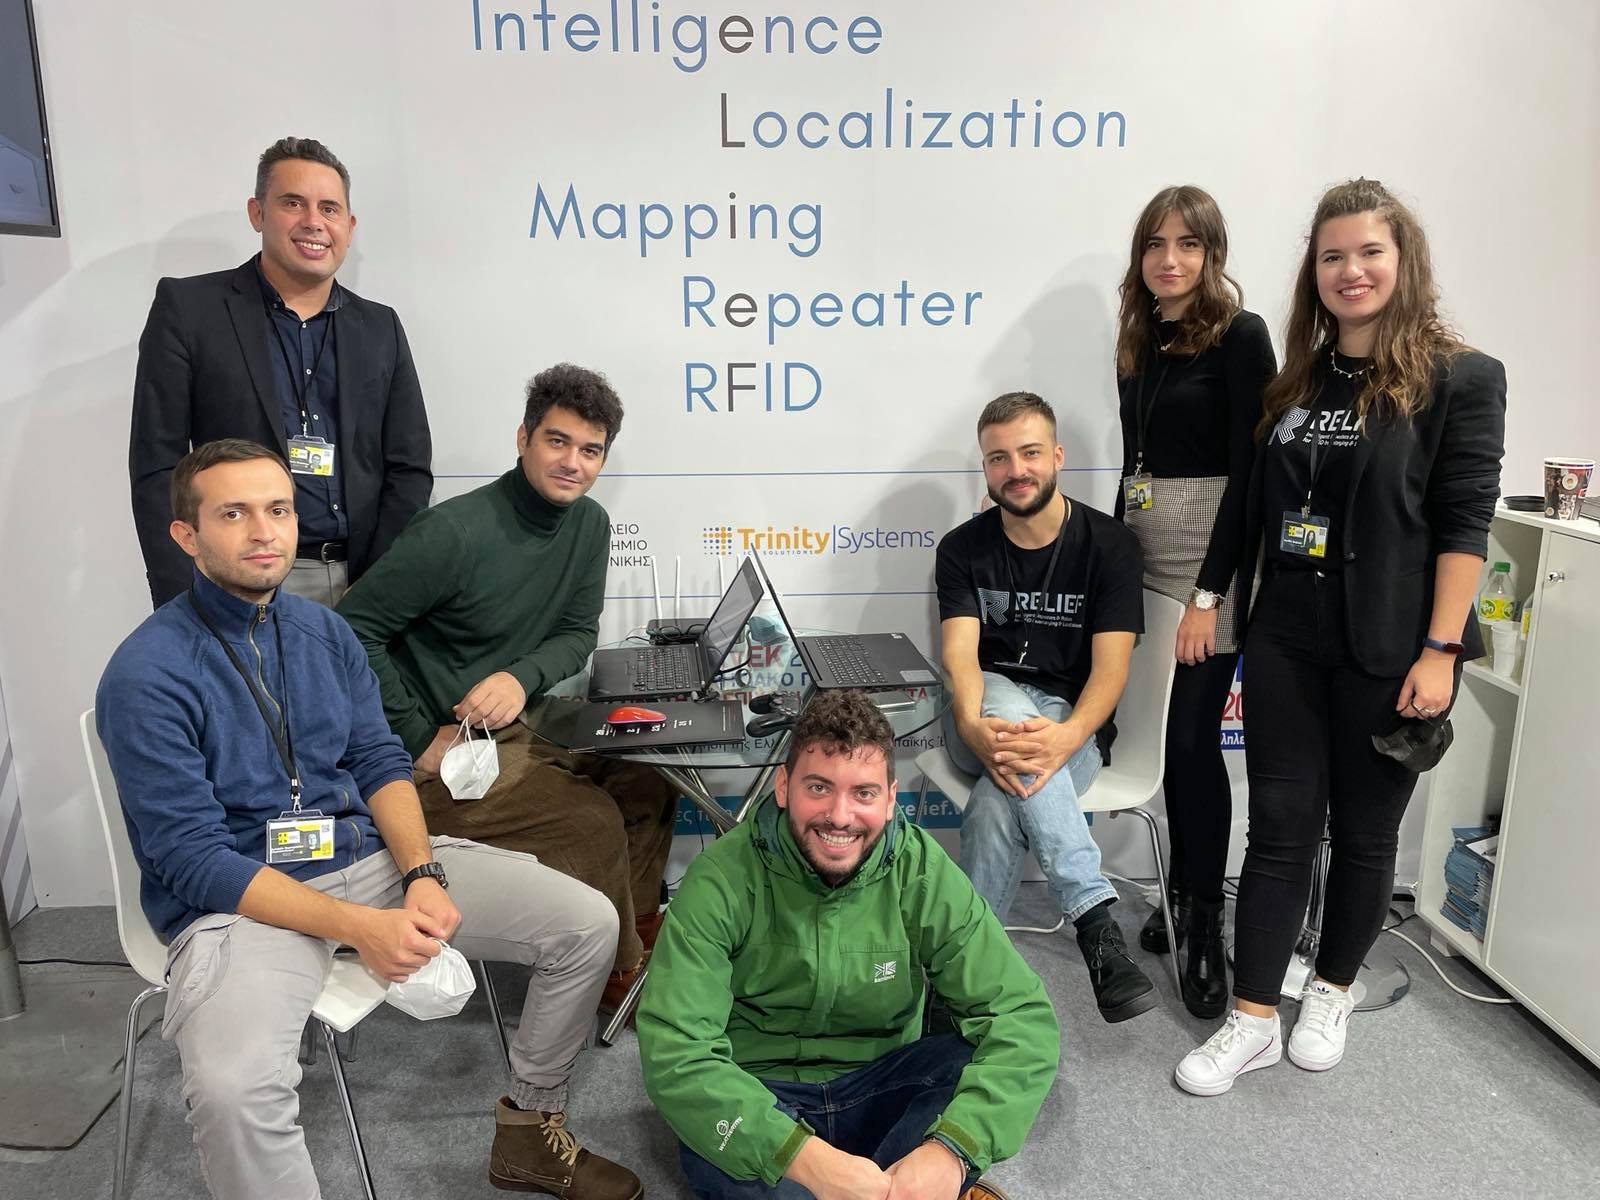
\includegraphics[scale=0.25]{./figures/parts/appendix/chapters/06/beyond_1.jpg}
  \caption{\small Από αριστερά προς δεξιά: Αντώνης Δημητρίου, Αριστείδης
           Ραπτόπουλος-Χατζηστεφάνου, Αλέξανδρος Φιλοθέου, Τάσος Τζιτζής,
           Σπύρος Μεγάλου, Ανδρεάνα Μάλαμα, Βασιλική Δρακάκη. Απούσα η
           Σταυρούλα Σιάχαλου}
\end{figure}
%%%%%%%%%%%%%%%%%%%%%%%%%%%%%%%%%%%%%%%%%%%%%%%%%%%%%%%%%%%%%%%%%%%%%%%%%%%%%%%%
\begin{figure}[H]\centering
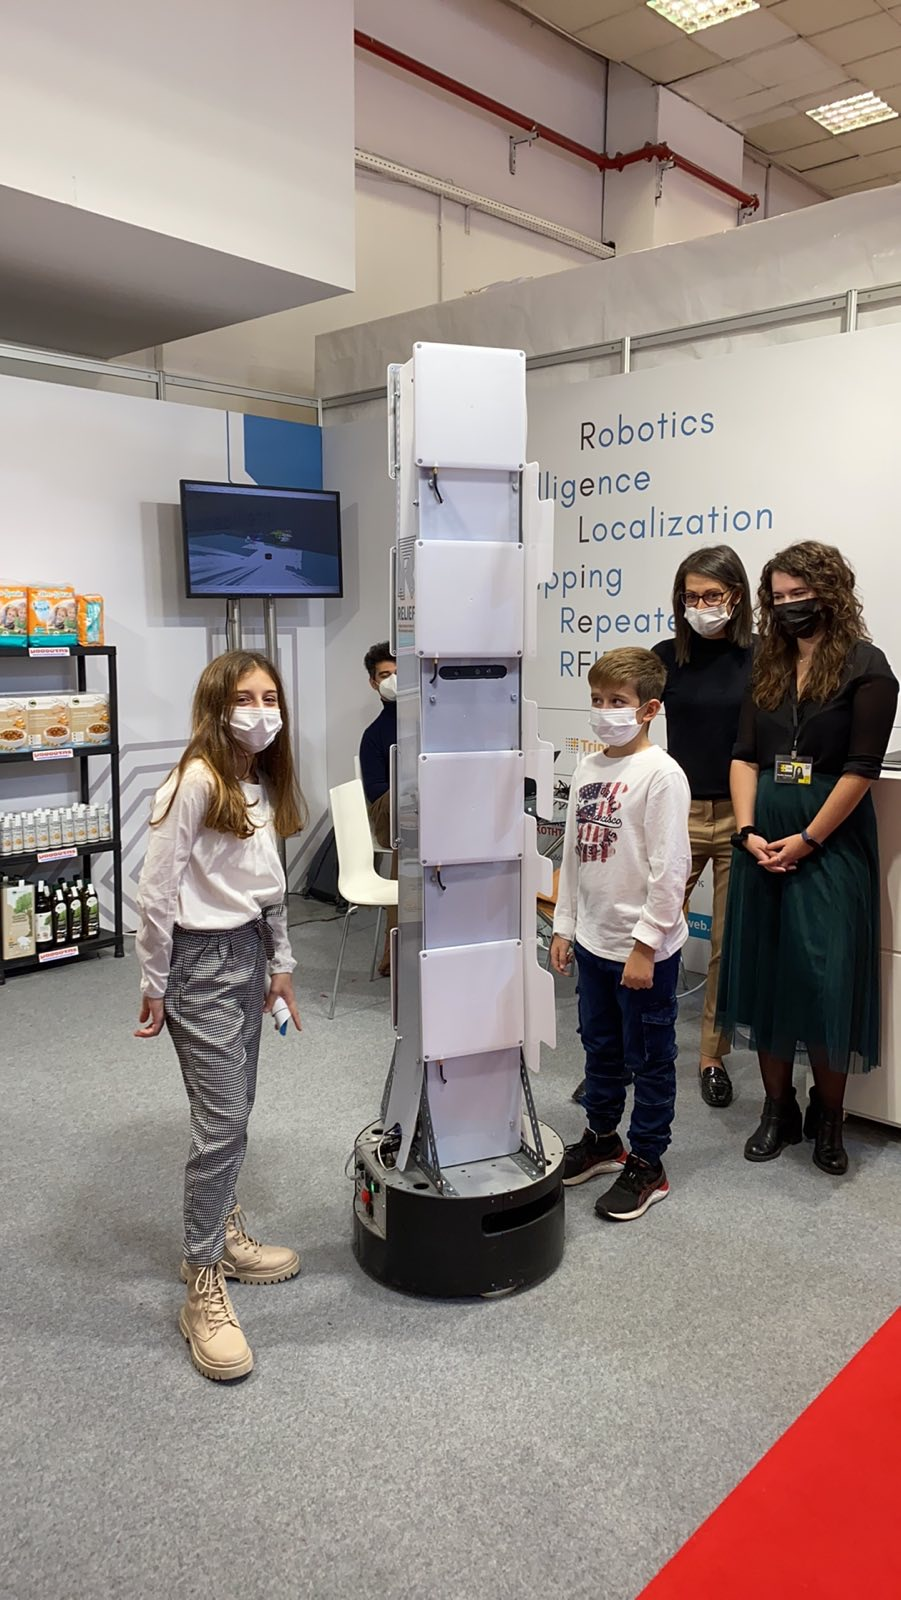
\includegraphics[scale=0.25]{./figures/parts/appendix/chapters/06/beyond_2.jpg}
  \caption{\small Το αγόρι κοιτάει το ρομπότ καχύποπτα. Πριν τραβηχθεί η
           φωτογραφία το ρομπότ περιστρέφετο επιτόπου επί ώρα, παρακολουθώντας
           το αγόρι, και κυνηγόντας τό όπου το πήγαινε---το αγόρι νόμιζε το
           ρομπότ ως αυτοδύναμο καθώς δεν είχε δει τον συγγραφέα να κρατάει
           στα χέρια του το χειριστήριό του}
\end{figure}
%%%%%%%%%%%%%%%%%%%%%%%%%%%%%%%%%%%%%%%%%%%%%%%%%%%%%%%%%%%%%%%%%%%%%%%%%%%%%%%%
\begin{figure}[H]\centering
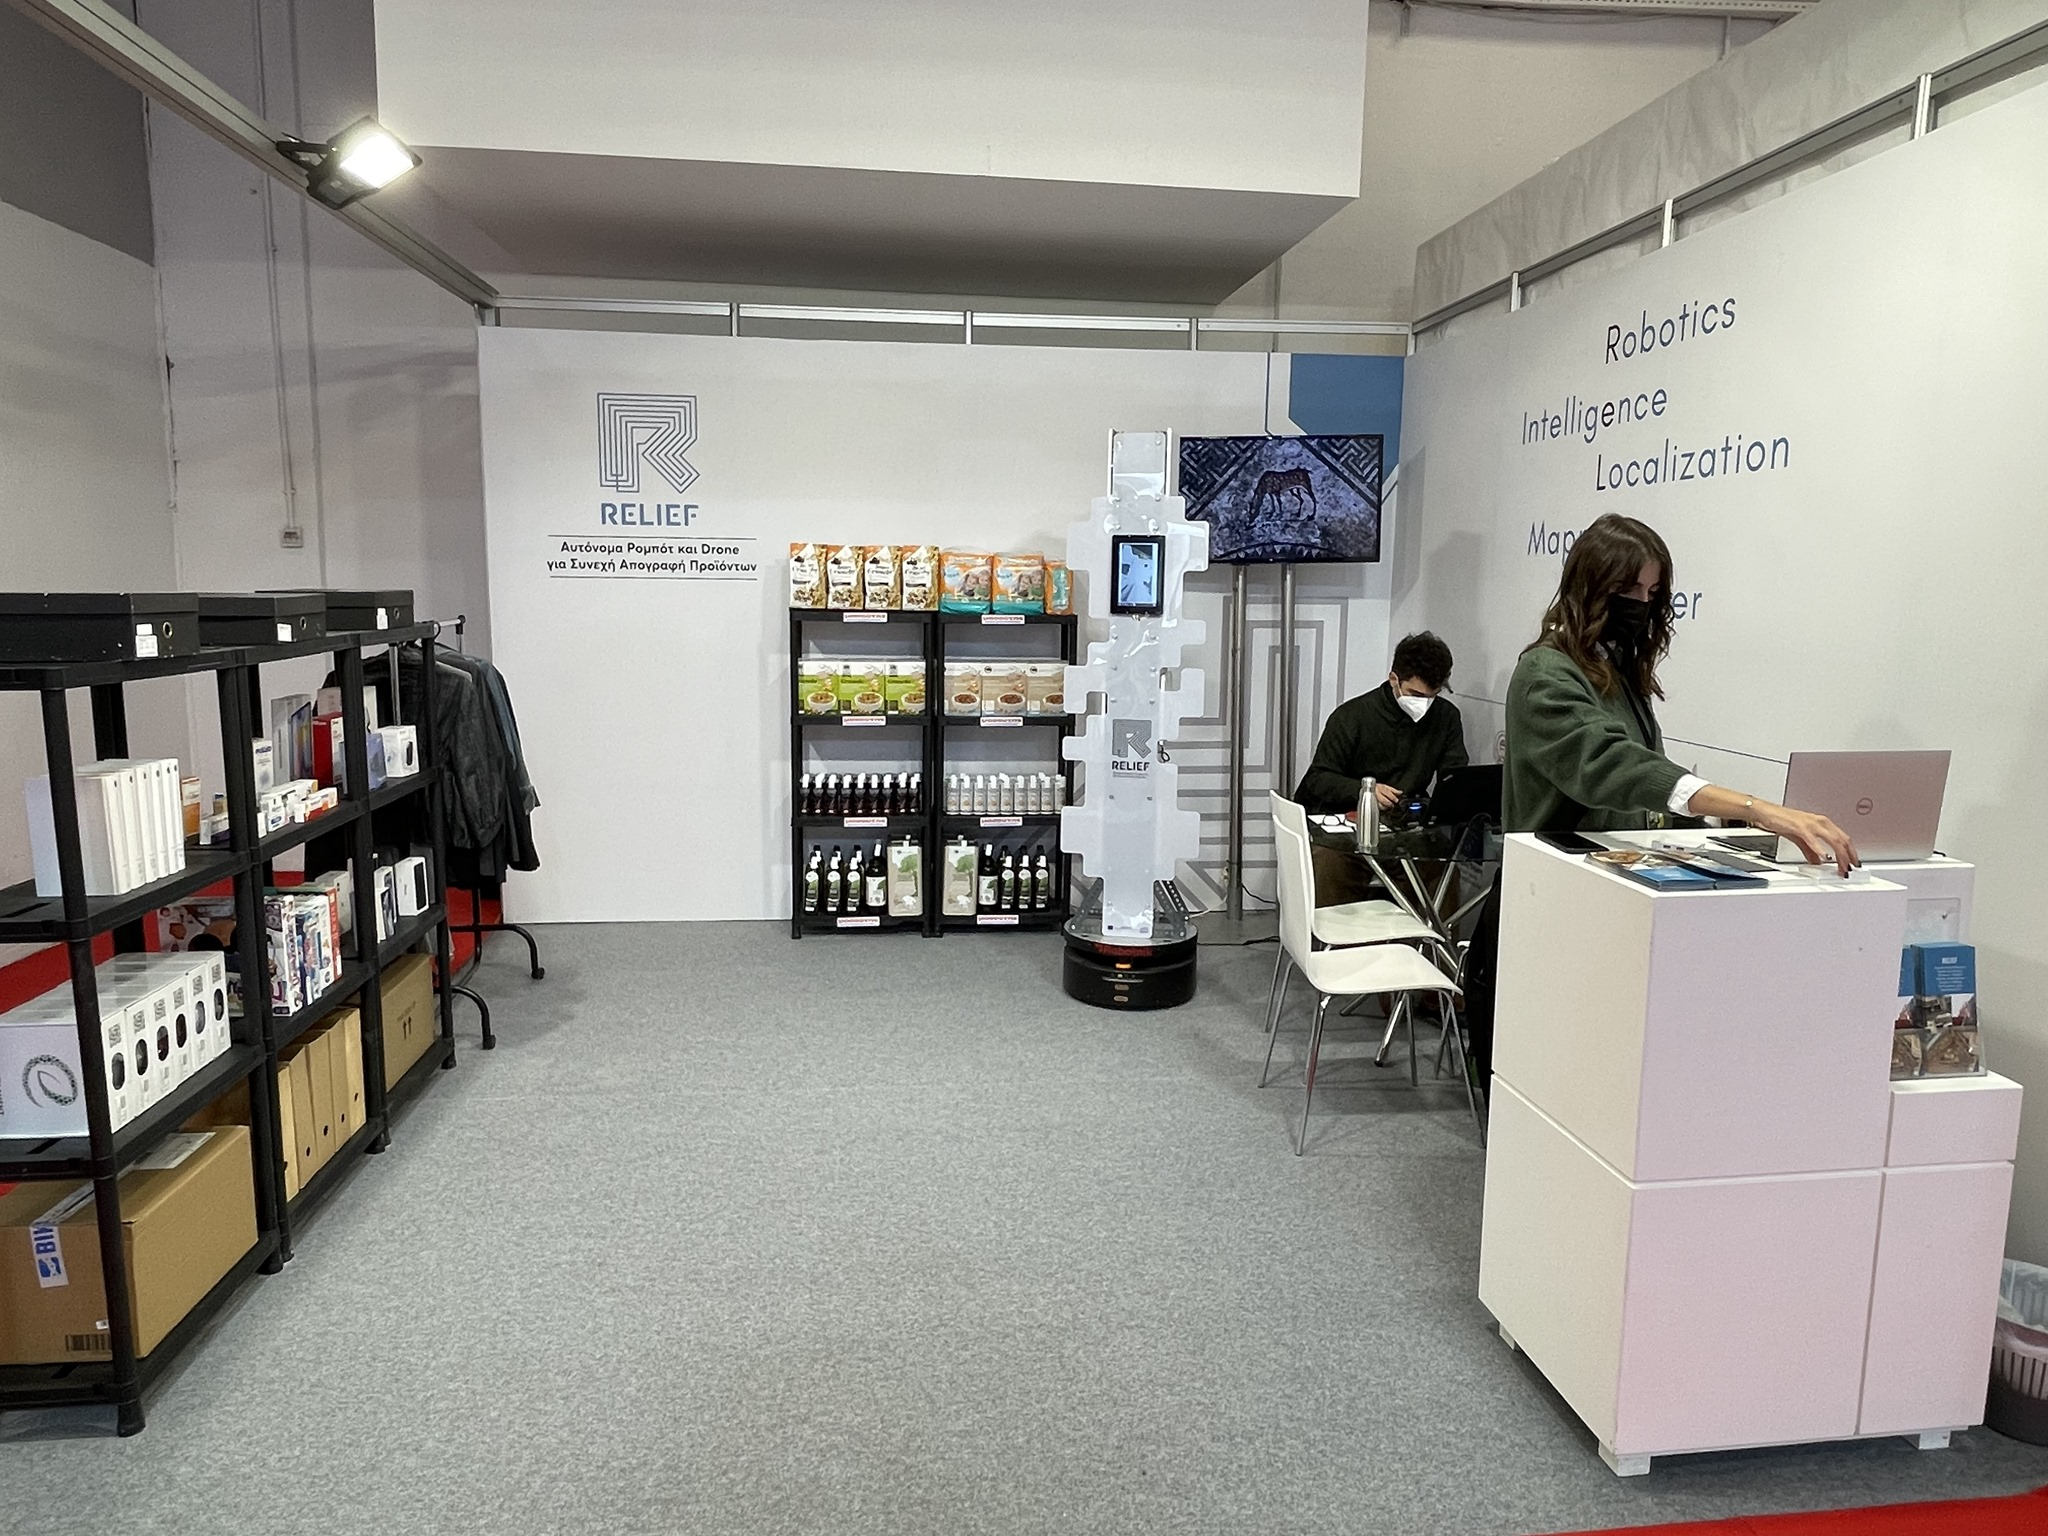
\includegraphics[scale=0.2]{./figures/parts/appendix/chapters/06/beyond_3.jpg}
  \caption{\small Σε κάποιο διάλειμμα από τα κοσμικά φώτα και τις επιδείξεις
           απογραφής προϊόντων και εύρεσης της θέσης τους μέσω τεχνολογίας RFID}
\end{figure}
%%%%%%%%%%%%%%%%%%%%%%%%%%%%%%%%%%%%%%%%%%%%%%%%%%%%%%%%%%%%%%%%%%%%%%%%%%%%%%%%
\begin{figure}[H]\centering
  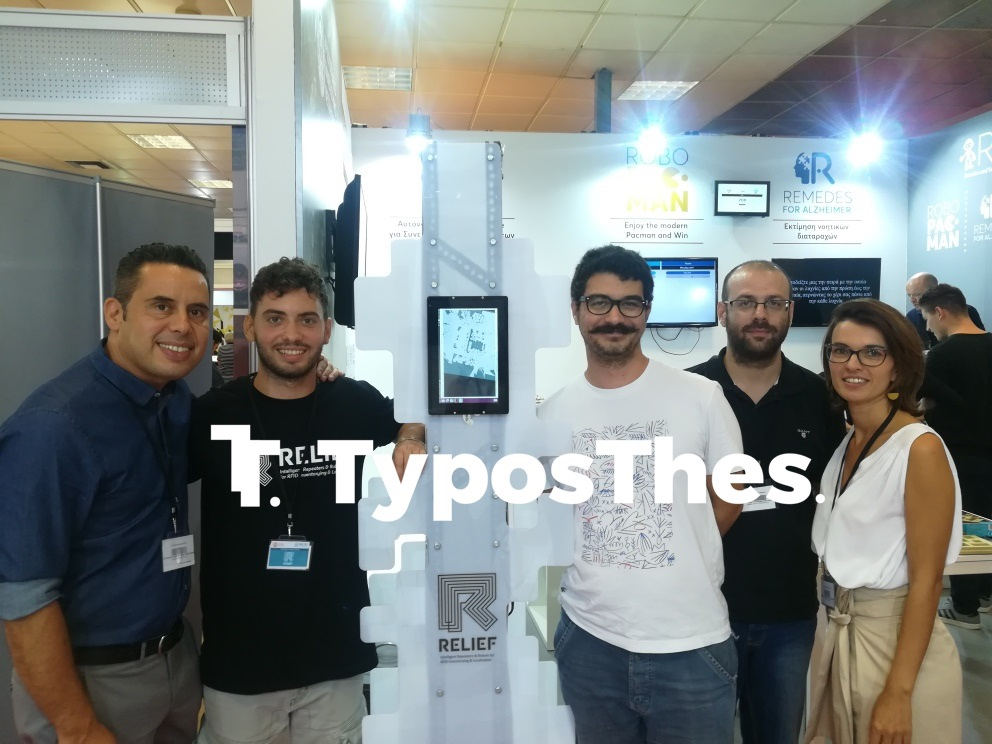
\includegraphics[scale=0.4]{./figures/parts/appendix/chapters/06/relief_begin.jpg}
  \caption{\small Στην αρχή: Το 2019 με το RB1 στη ΔΕΘ. Ένα χρόνο μετά την
           εκκίνηση του έργου RELIEF. Από αριστερά προς τα δεξιά: Αντώνης
           Δημητρίου, Τάσος Τζιτζής, Αλέξανδρος Φιλοθέου, Μάνος Τσαρδούλιας,
           Σταυρούλα Σιάχαλου}
  \vspace{1cm}
  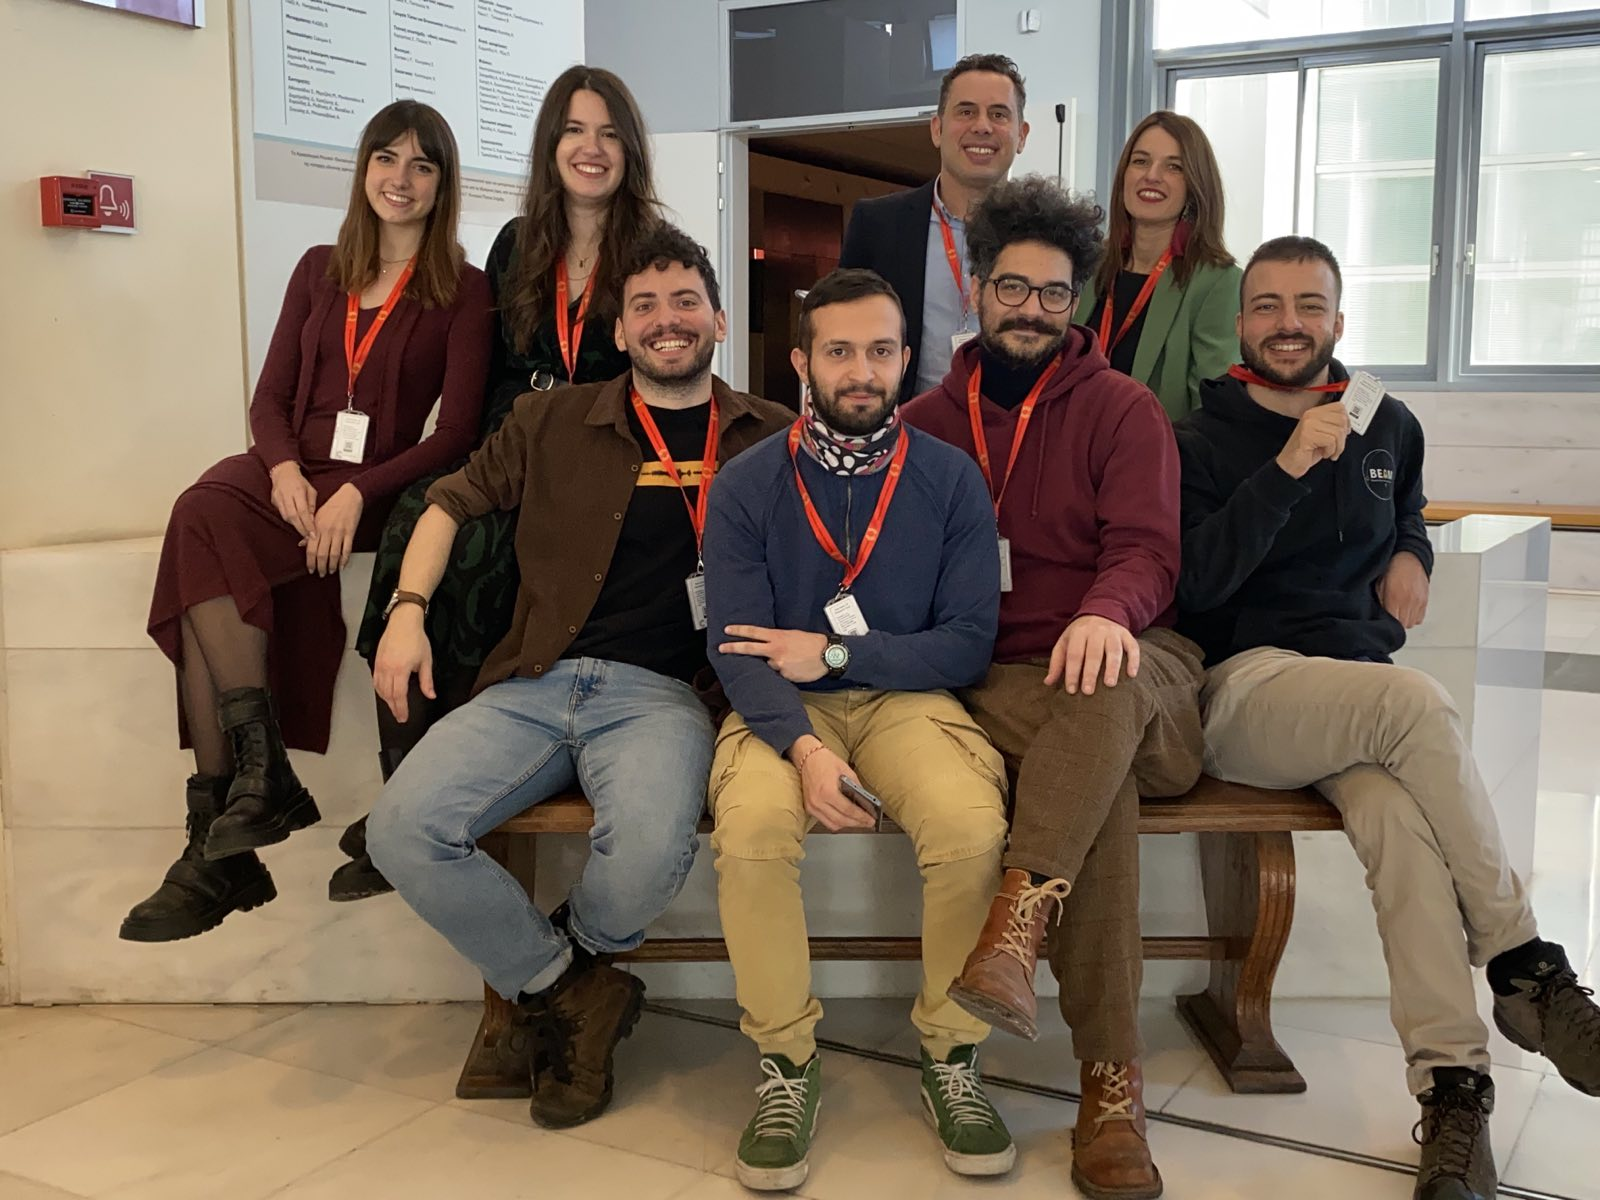
\includegraphics[scale=0.25]{./figures/parts/appendix/chapters/06/cultureid_end.jpg}
  \caption{\small Στο τέλος: Στην ημερίδα παρουσίασης των αποτελεσμάτων του
           έργου CULTUREID στις 17 Μαρτίου 2023}
\end{figure}


%%%%%%%%%%%%%%%%%%%%%%%%%%%%%%%%%%%%%%%%%%%%%%%%%%%%%%%%%%%%%%%%%%%%%%%%%%%%%%%%
\section{Η ρομποτική κολεκσιόν φθινόπωρο 2018-άνοιξη 2023}
%%%%%%%%%%%%%%%%%%%%%%%%%%%%%%%%%%%%%%%%%%%%%%%%%%%%%%%%%%%%%%%%%%%%%%%%%%%%%%%%
\begin{figure}[H]\centering
  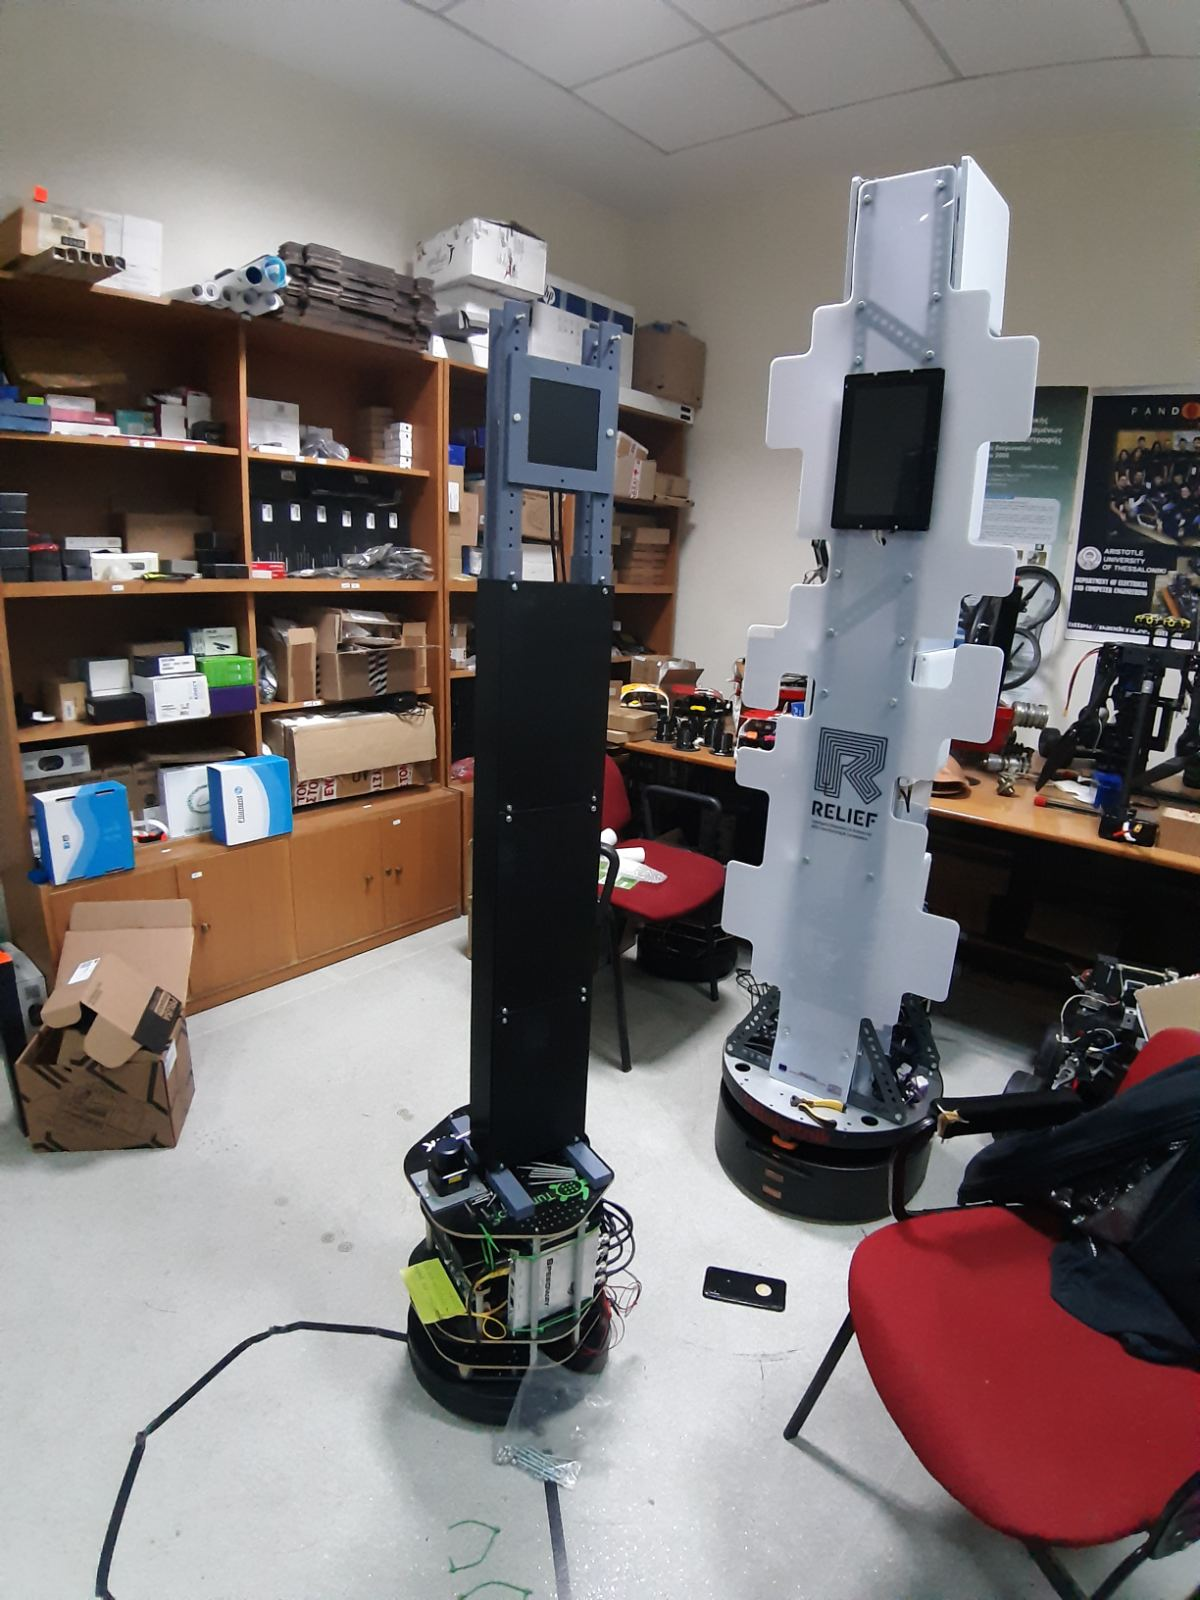
\includegraphics[scale=0.25]{./figures/parts/appendix/chapters/06/relief_robots.jpg}
  \caption{\small Το μεγάλο και το μαύρο ρομπότ του έργου RELIEF}
\end{figure}
%%%%%%%%%%%%%%%%%%%%%%%%%%%%%%%%%%%%%%%%%%%%%%%%%%%%%%%%%%%%%%%%%%%%%%%%%%%%%%%%
\begin{figure}[H]\centering
  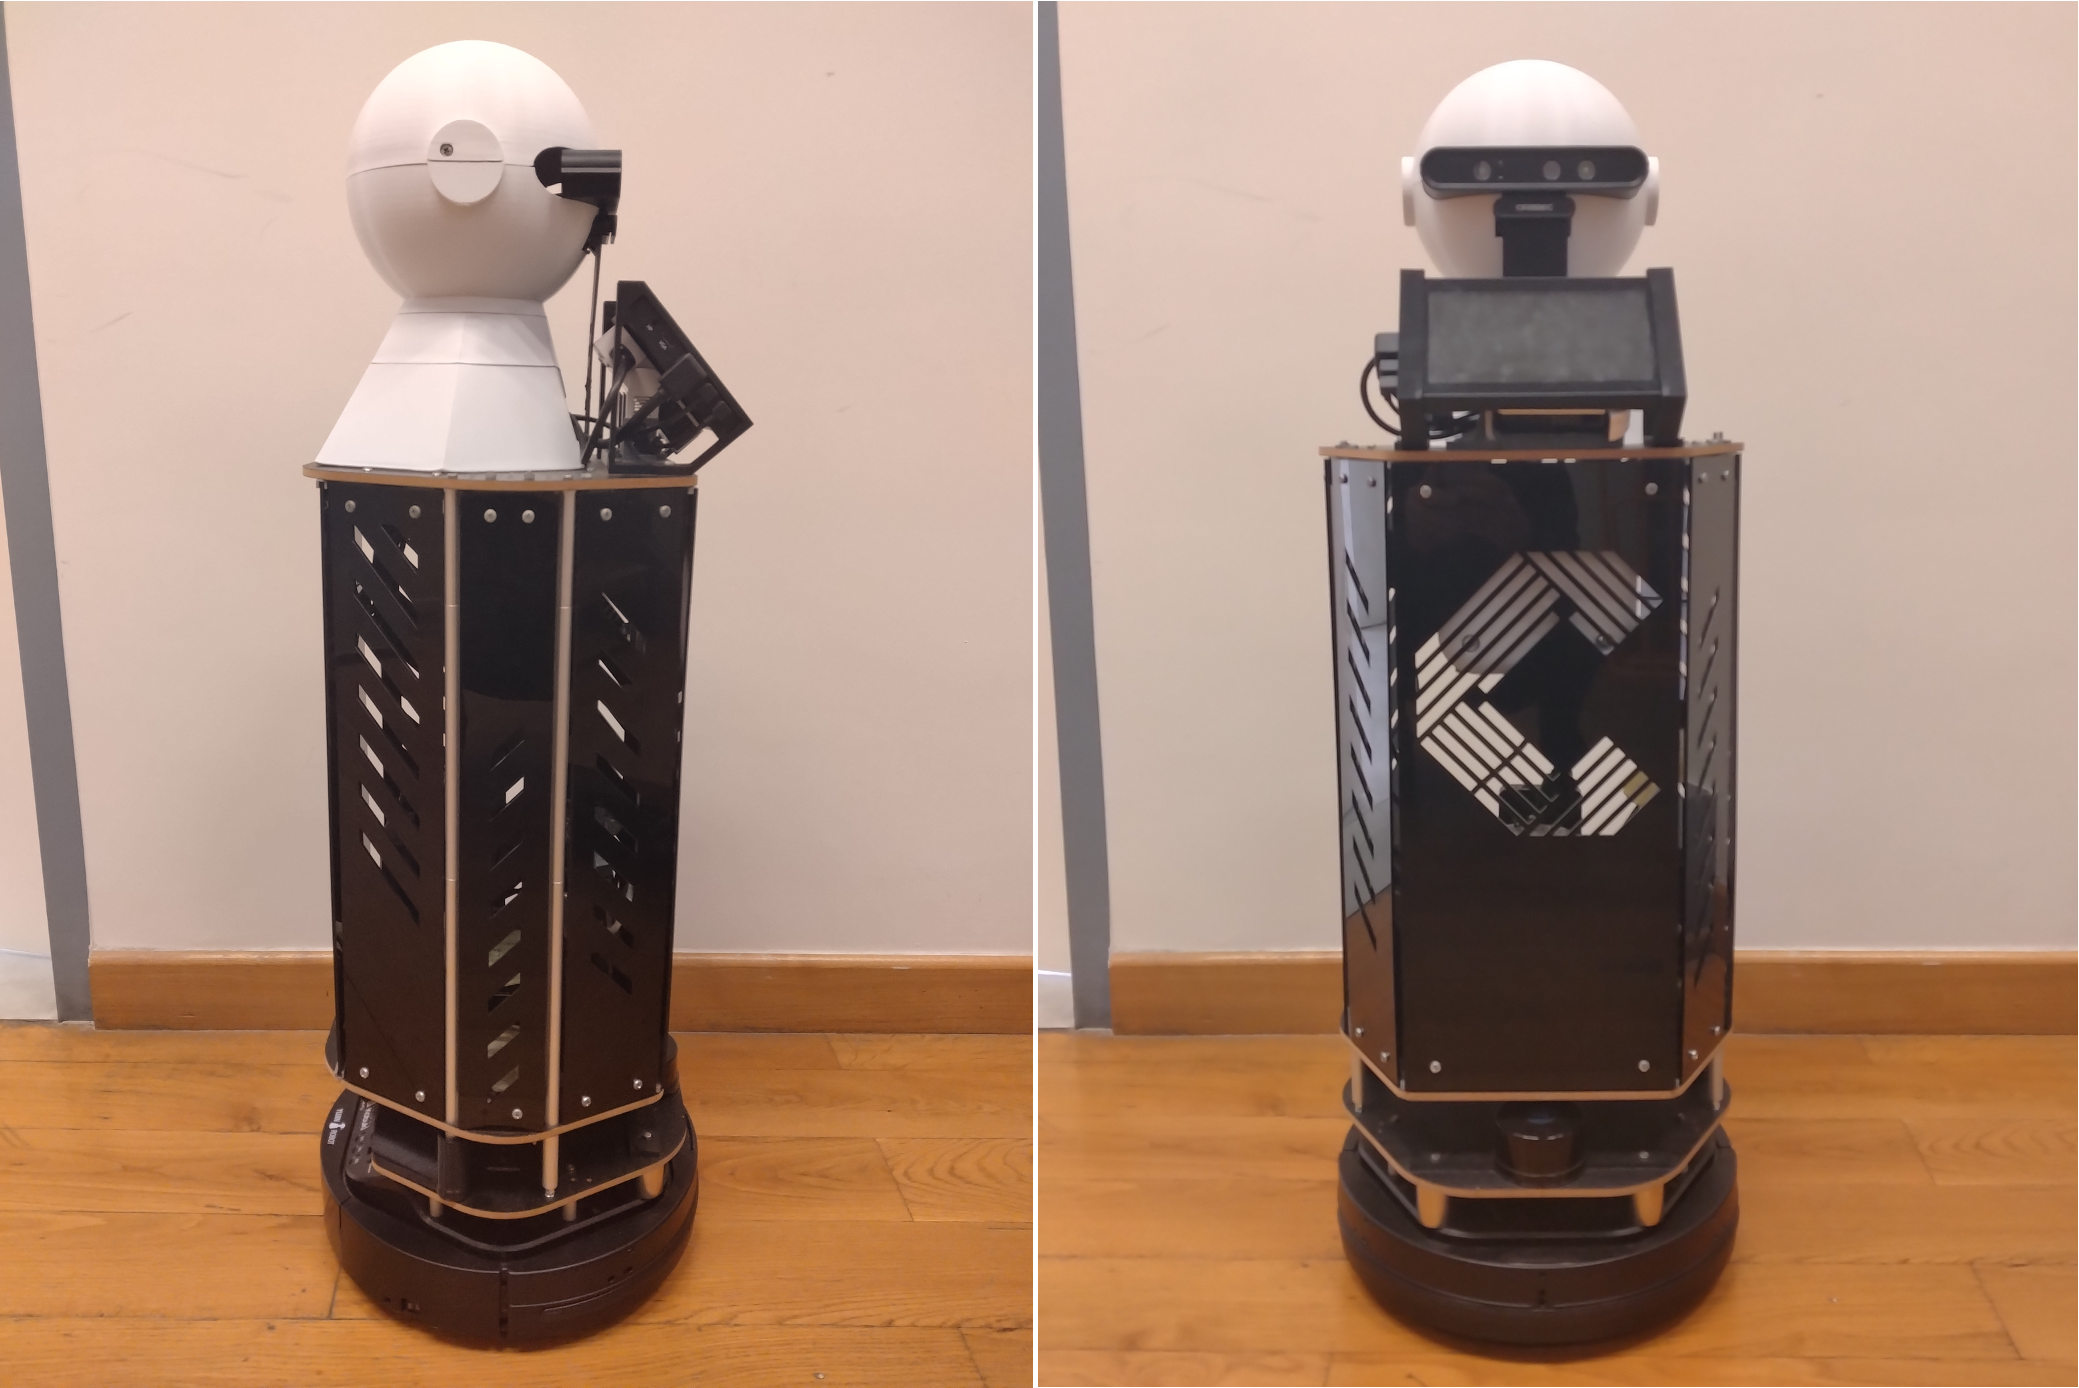
\includegraphics[scale=0.2]{./figures/parts/appendix/chapters/06/indy.png}
  \caption{\small Ο indy του έργου CULTUREID}
\end{figure}
%%%%%%%%%%%%%%%%%%%%%%%%%%%%%%%%%%%%%%%%%%%%%%%%%%%%%%%%%%%%%%%%%%%%%%%%%%%%%%%%
\begin{figure}[H]\centering
  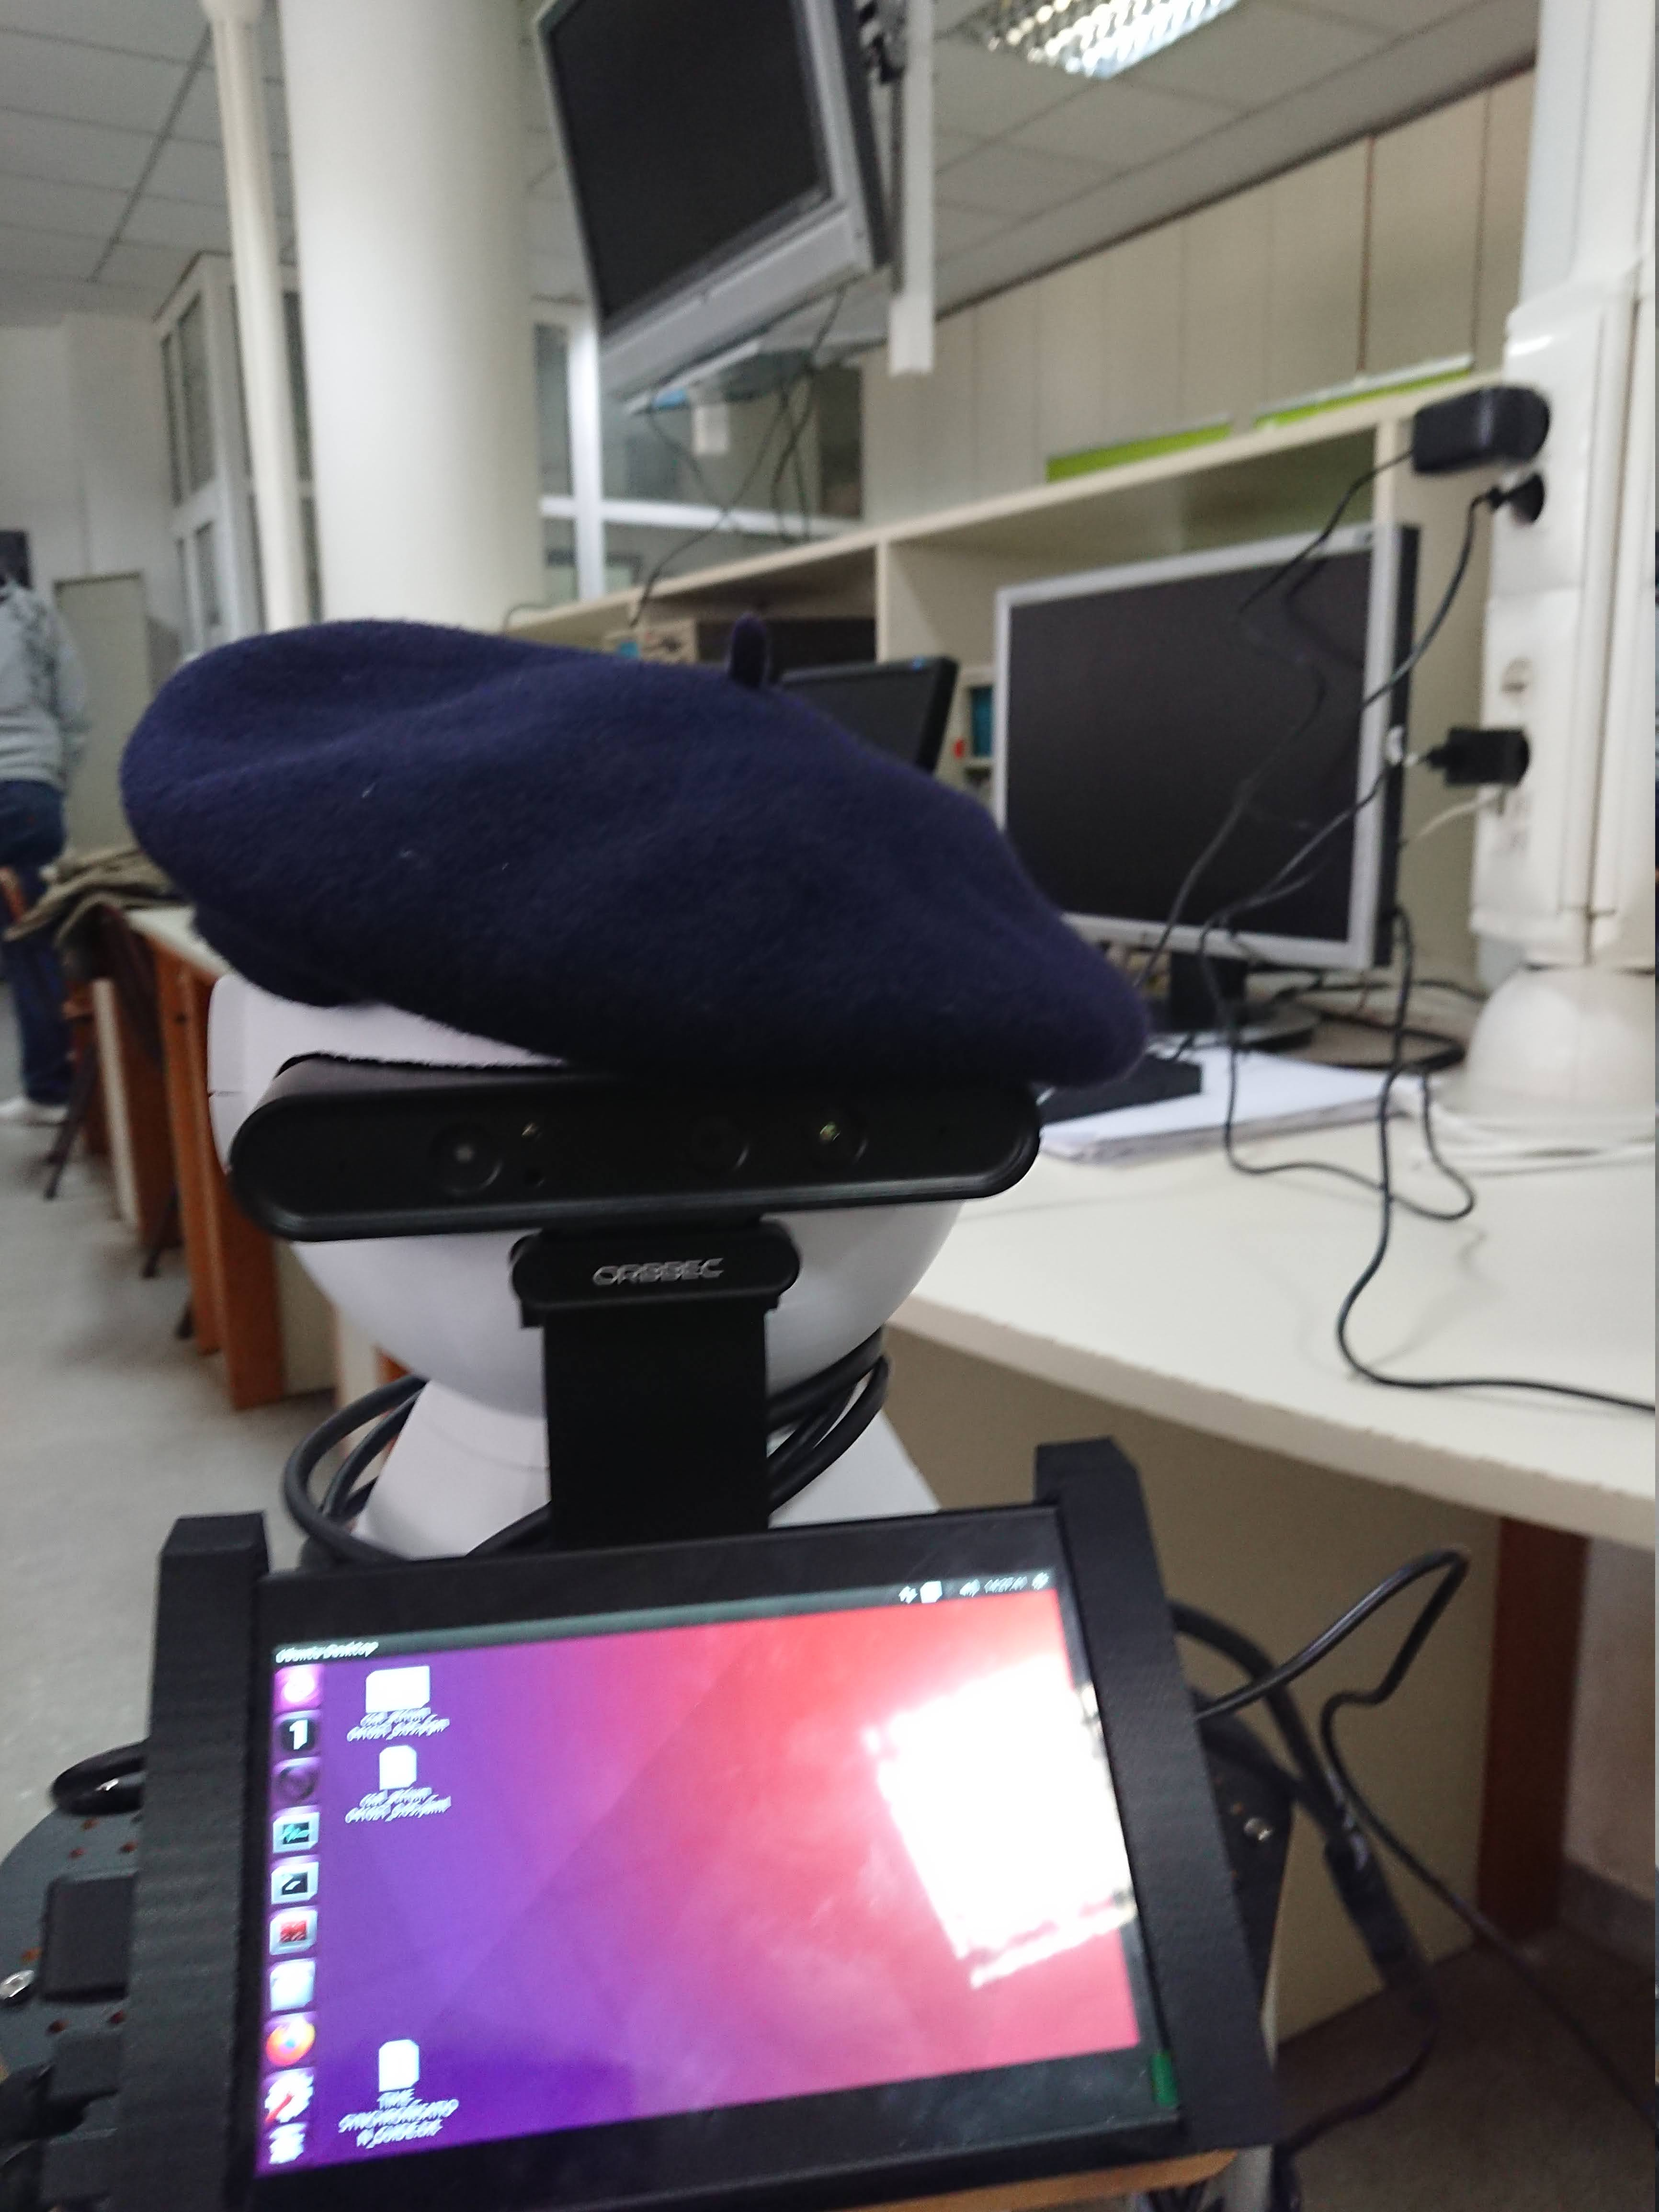
\includegraphics[scale=0.1]{./figures/parts/appendix/chapters/06/indee.jpg}
  \caption{\small Ο indy CULTUREIDάρης}
\end{figure}



%%%%%%%%%%%%%%%%%%%%%%%%%%%%%%%%%%%%%%%%%%%%%%%%%%%%%%%%%%%%%%%%%%%%%%%%%%%%%%%%
\section{Ρομπότ και Αρχαιολογικό Μουσείο Θεσσαλονίκης}
%%%%%%%%%%%%%%%%%%%%%%%%%%%%%%%%%%%%%%%%%%%%%%%%%%%%%%%%%%%%%%%%%%%%%%%%%%%%%%%%
\begin{figure}[H]\centering
  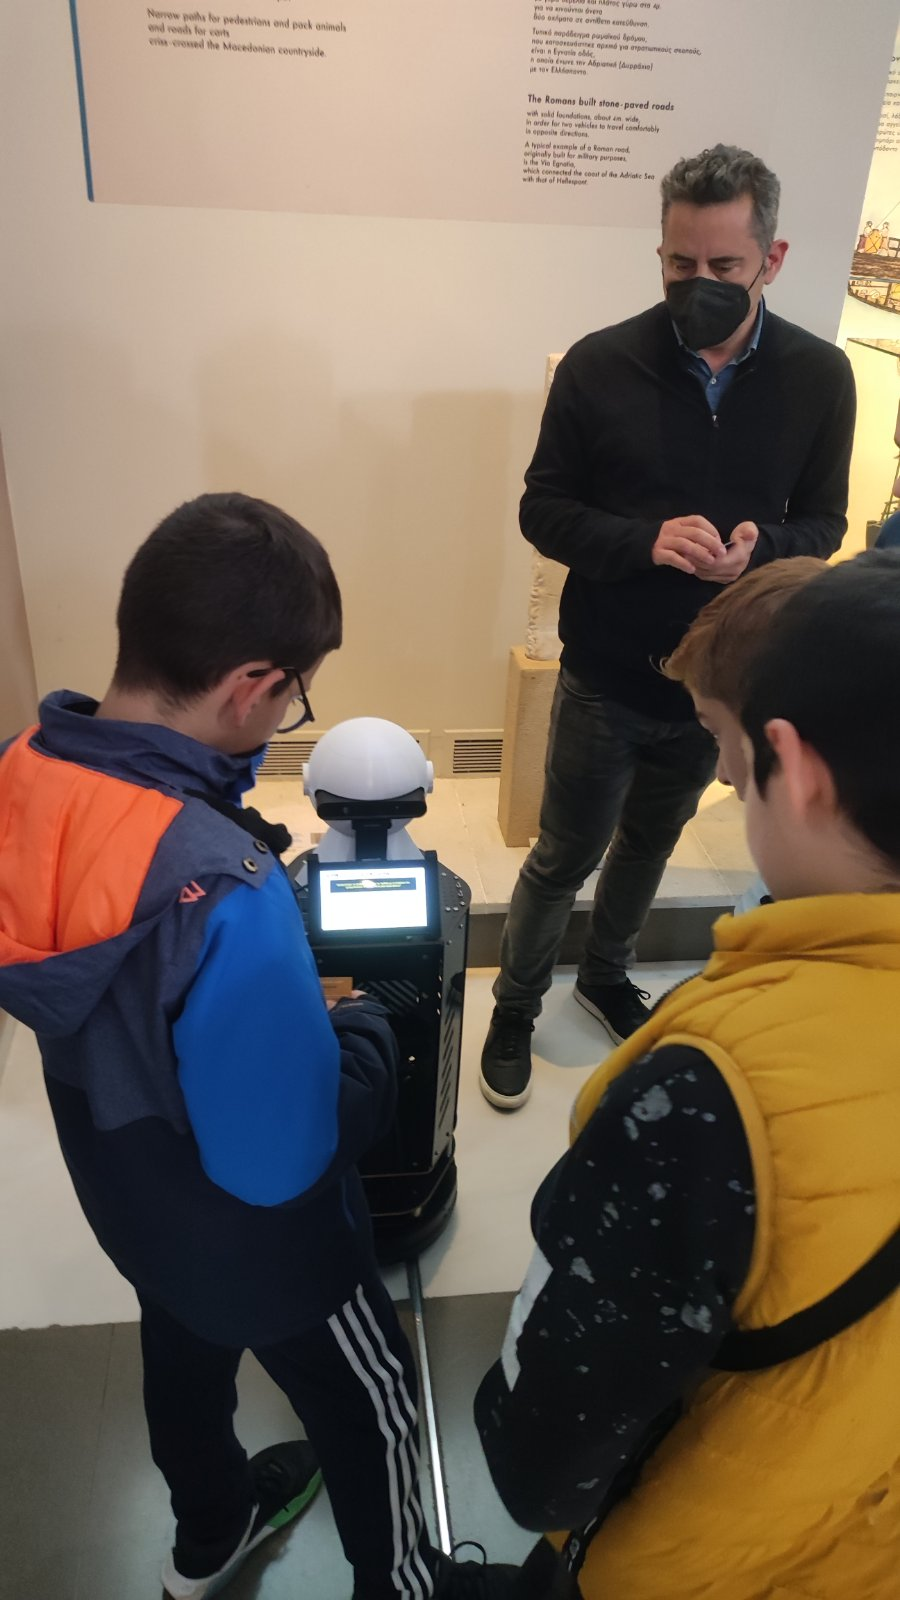
\includegraphics[scale=0.25]{./figures/parts/appendix/chapters/06/indy_at_museum.jpg}
  \caption{\small Ο indy επί τω έργω στο Αρχαιολογικό Μουσείο Θεσσαλονίκης}
\end{figure}
%%%%%%%%%%%%%%%%%%%%%%%%%%%%%%%%%%%%%%%%%%%%%%%%%%%%%%%%%%%%%%%%%%%%%%%%%%%%%%%%
\begin{figure}[H]\centering
  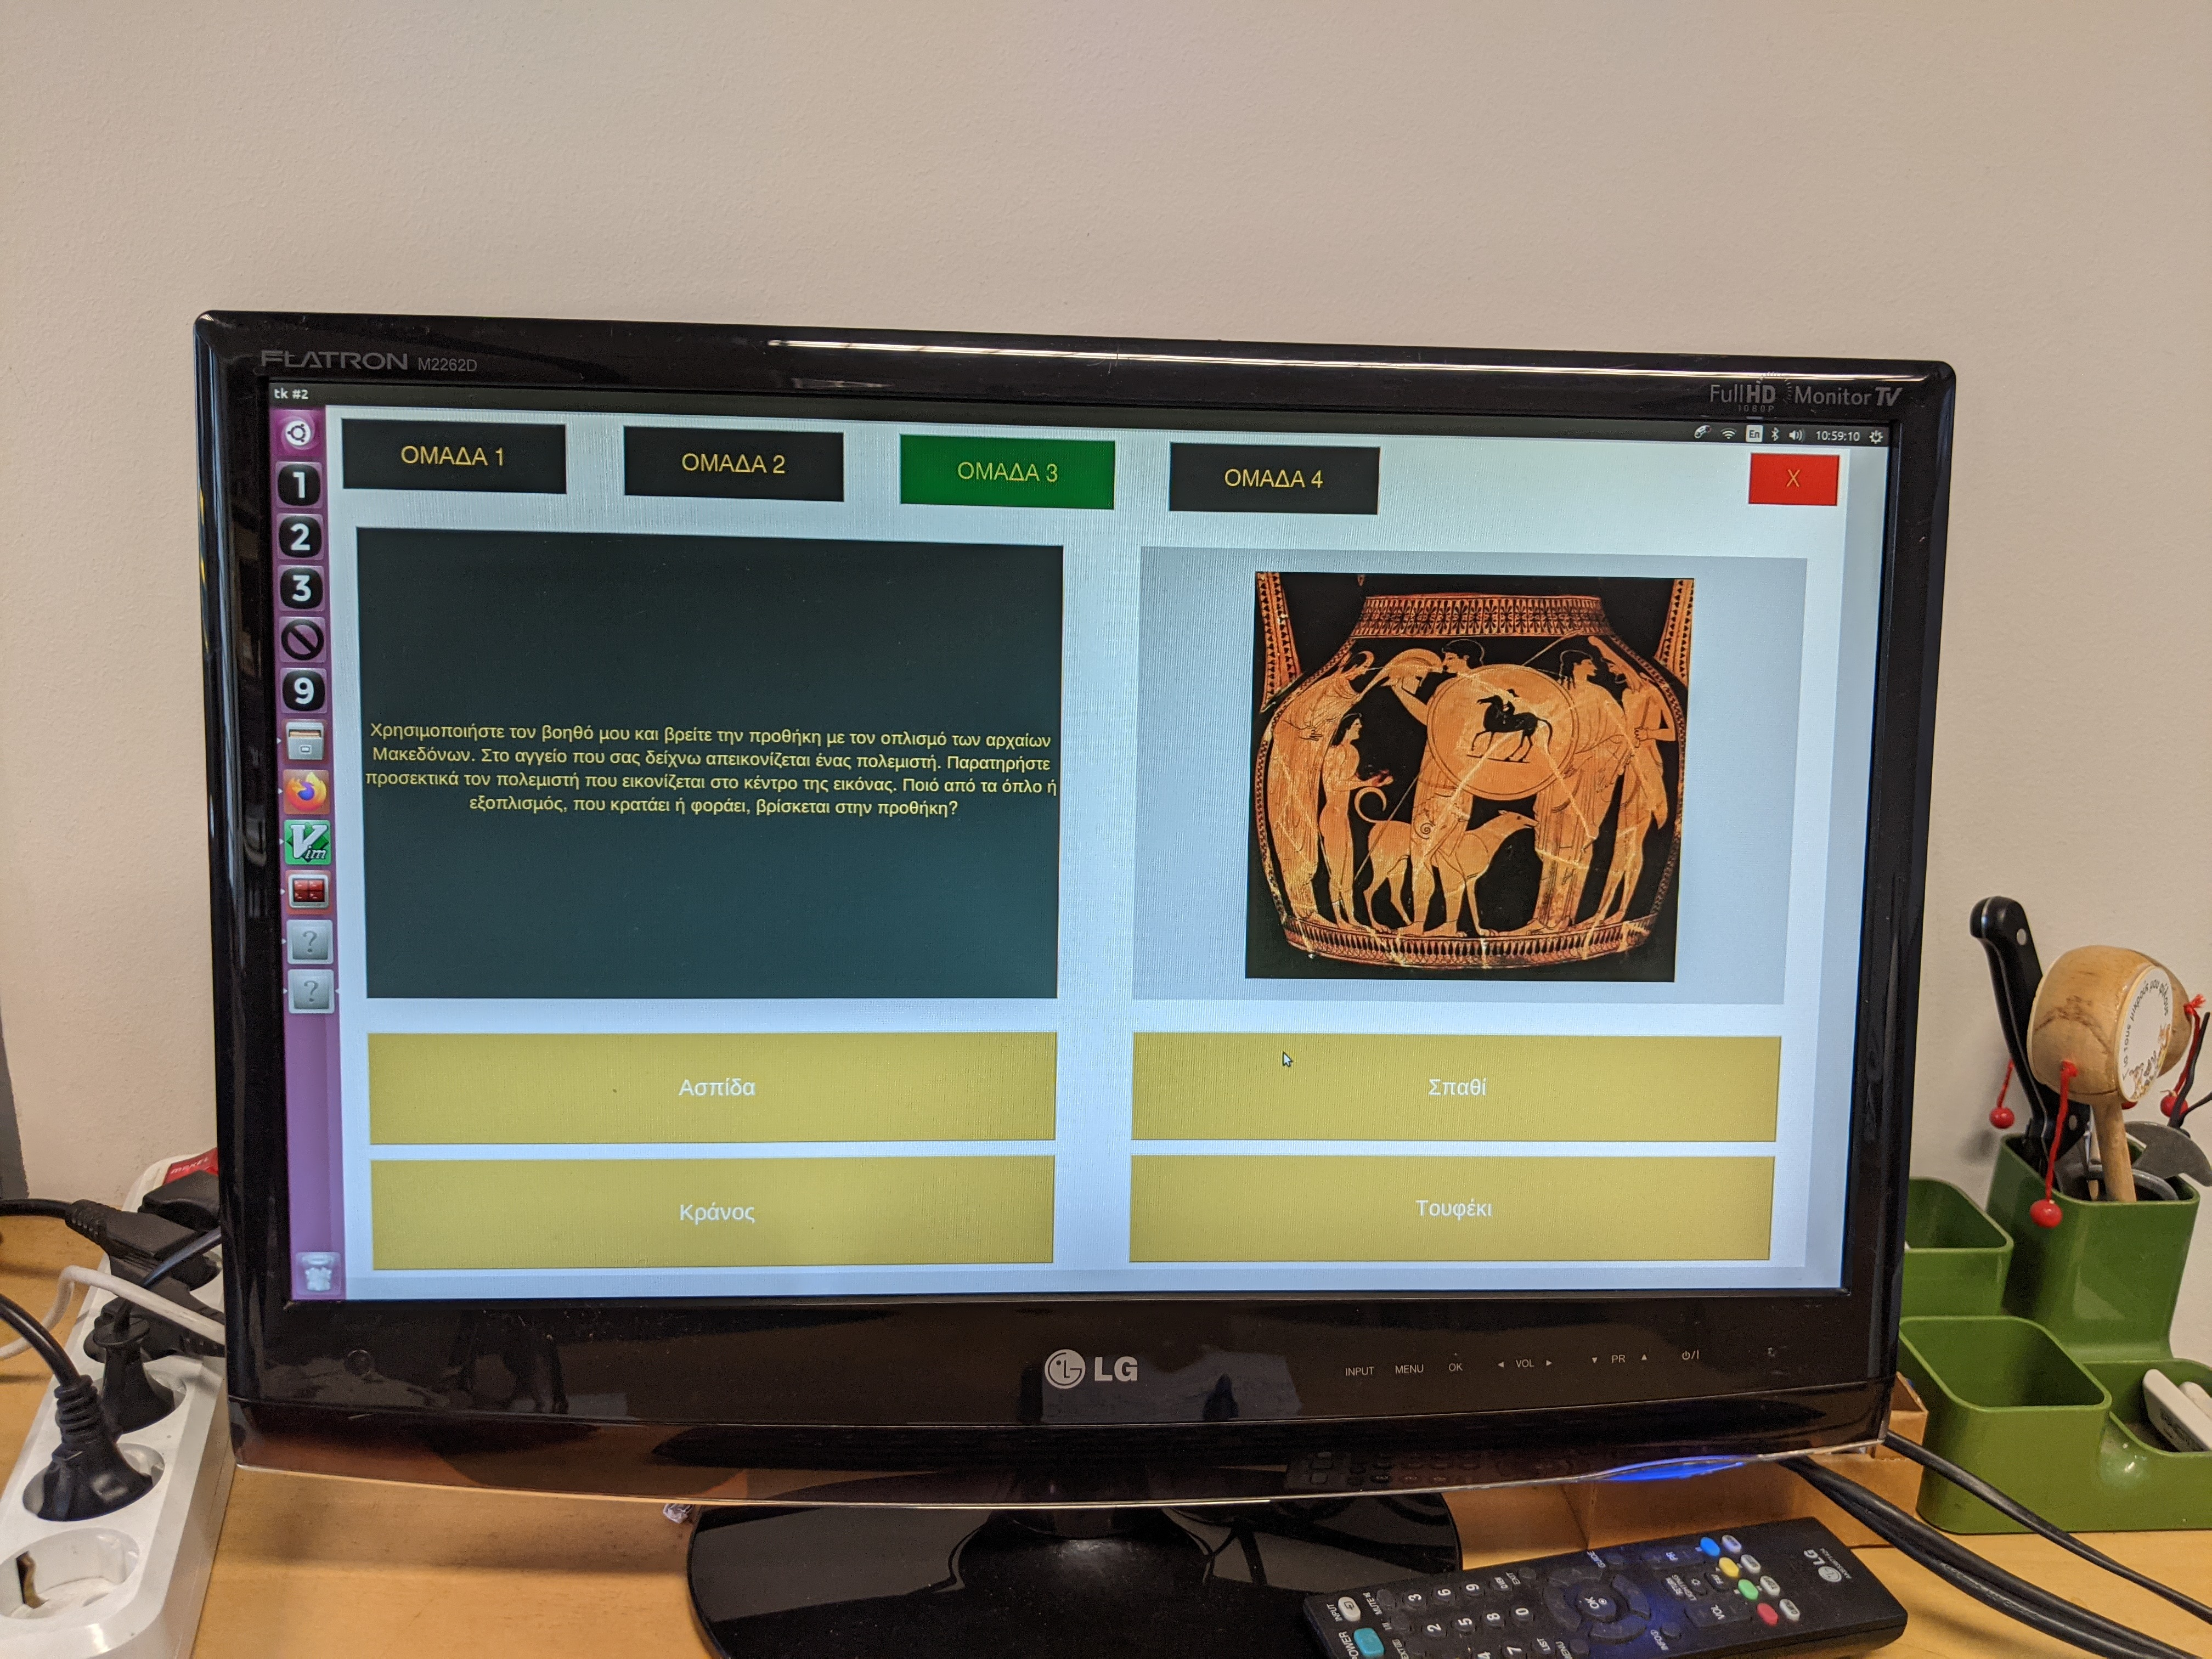
\includegraphics[scale=1]{./figures/parts/appendix/chapters/06/mouseio_1.jpg}
\end{figure}
%%%%%%%%%%%%%%%%%%%%%%%%%%%%%%%%%%%%%%%%%%%%%%%%%%%%%%%%%%%%%%%%%%%%%%%%%%%%%%%%
\begin{figure}[H]\centering
  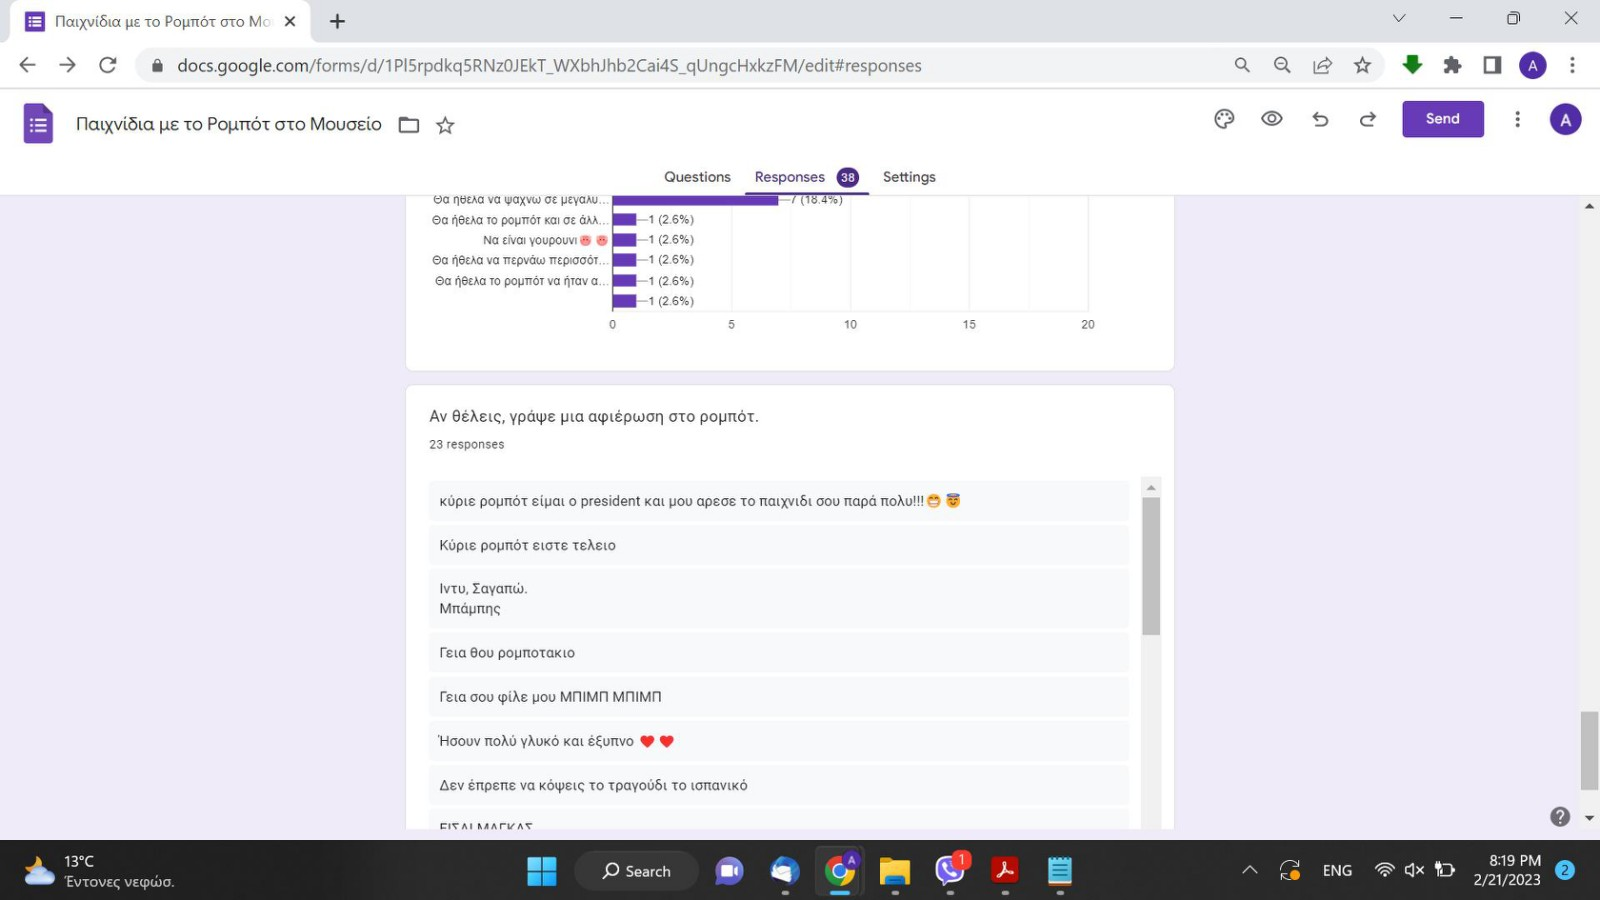
\includegraphics[scale=0.4]{./figures/parts/appendix/chapters/06/indy_kids_1.jpg}
\end{figure}
%%%%%%%%%%%%%%%%%%%%%%%%%%%%%%%%%%%%%%%%%%%%%%%%%%%%%%%%%%%%%%%%%%%%%%%%%%%%%%%%
\begin{figure}[H]\centering
  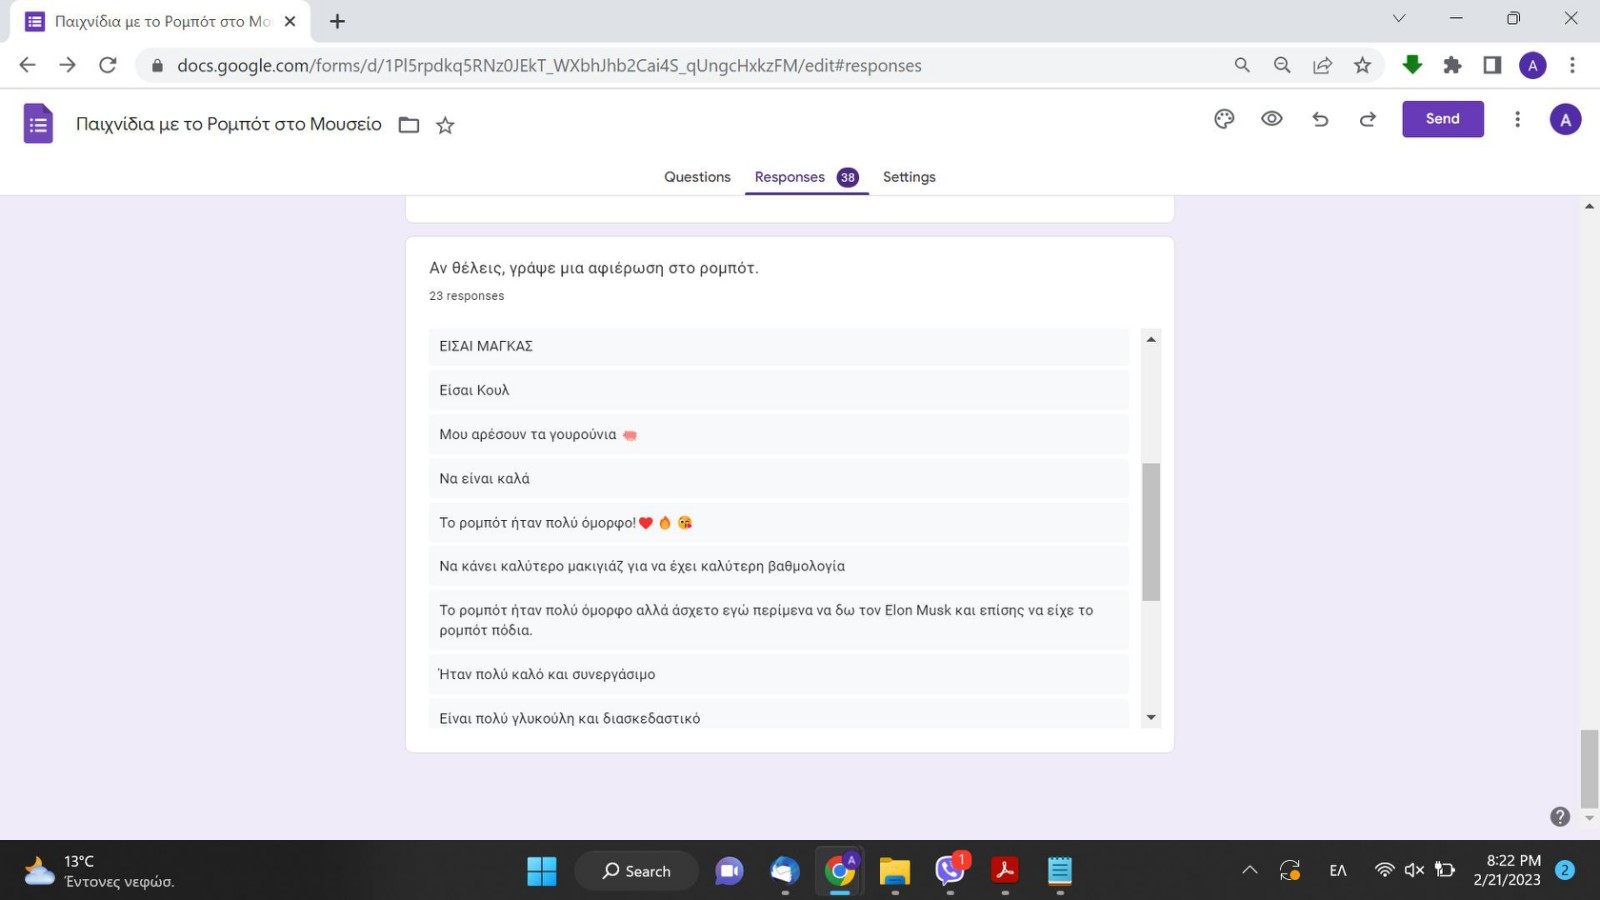
\includegraphics[scale=0.4]{./figures/parts/appendix/chapters/06/indy_kids_2.jpg}
\end{figure}
%%%%%%%%%%%%%%%%%%%%%%%%%%%%%%%%%%%%%%%%%%%%%%%%%%%%%%%%%%%%%%%%%%%%%%%%%%%%%%%%
\begin{figure}[H]\centering
  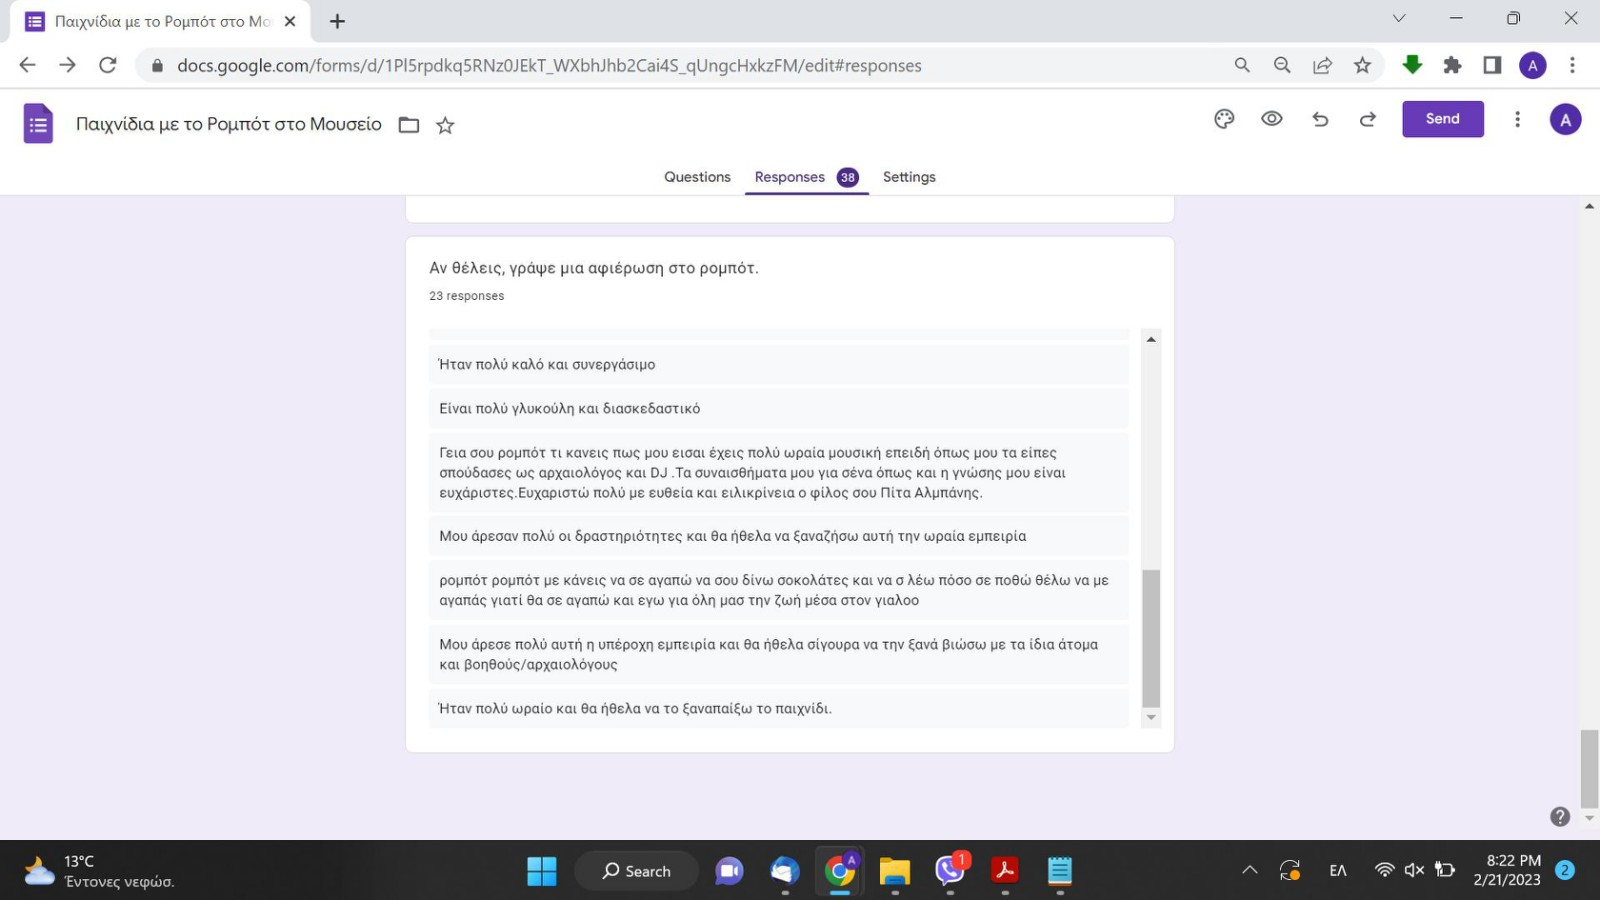
\includegraphics[scale=0.4]{./figures/parts/appendix/chapters/06/indy_kids_3.jpg}
\end{figure}

%%%%%%%%%%%%%%%%%%%%%%%%%%%%%%%%%%%%%%%%%%%%%%%%%%%%%%%%%%%%%%%%%%%%%%%%%%%%%%%%
\section{Το ταξίδι στην Ιαπωνία}
%%%%%%%%%%%%%%%%%%%%%%%%%%%%%%%%%%%%%%%%%%%%%%%%%%%%%%%%%%%%%%%%%%%%%%%%%%%%%%%%
\begin{figure}[H]\centering
  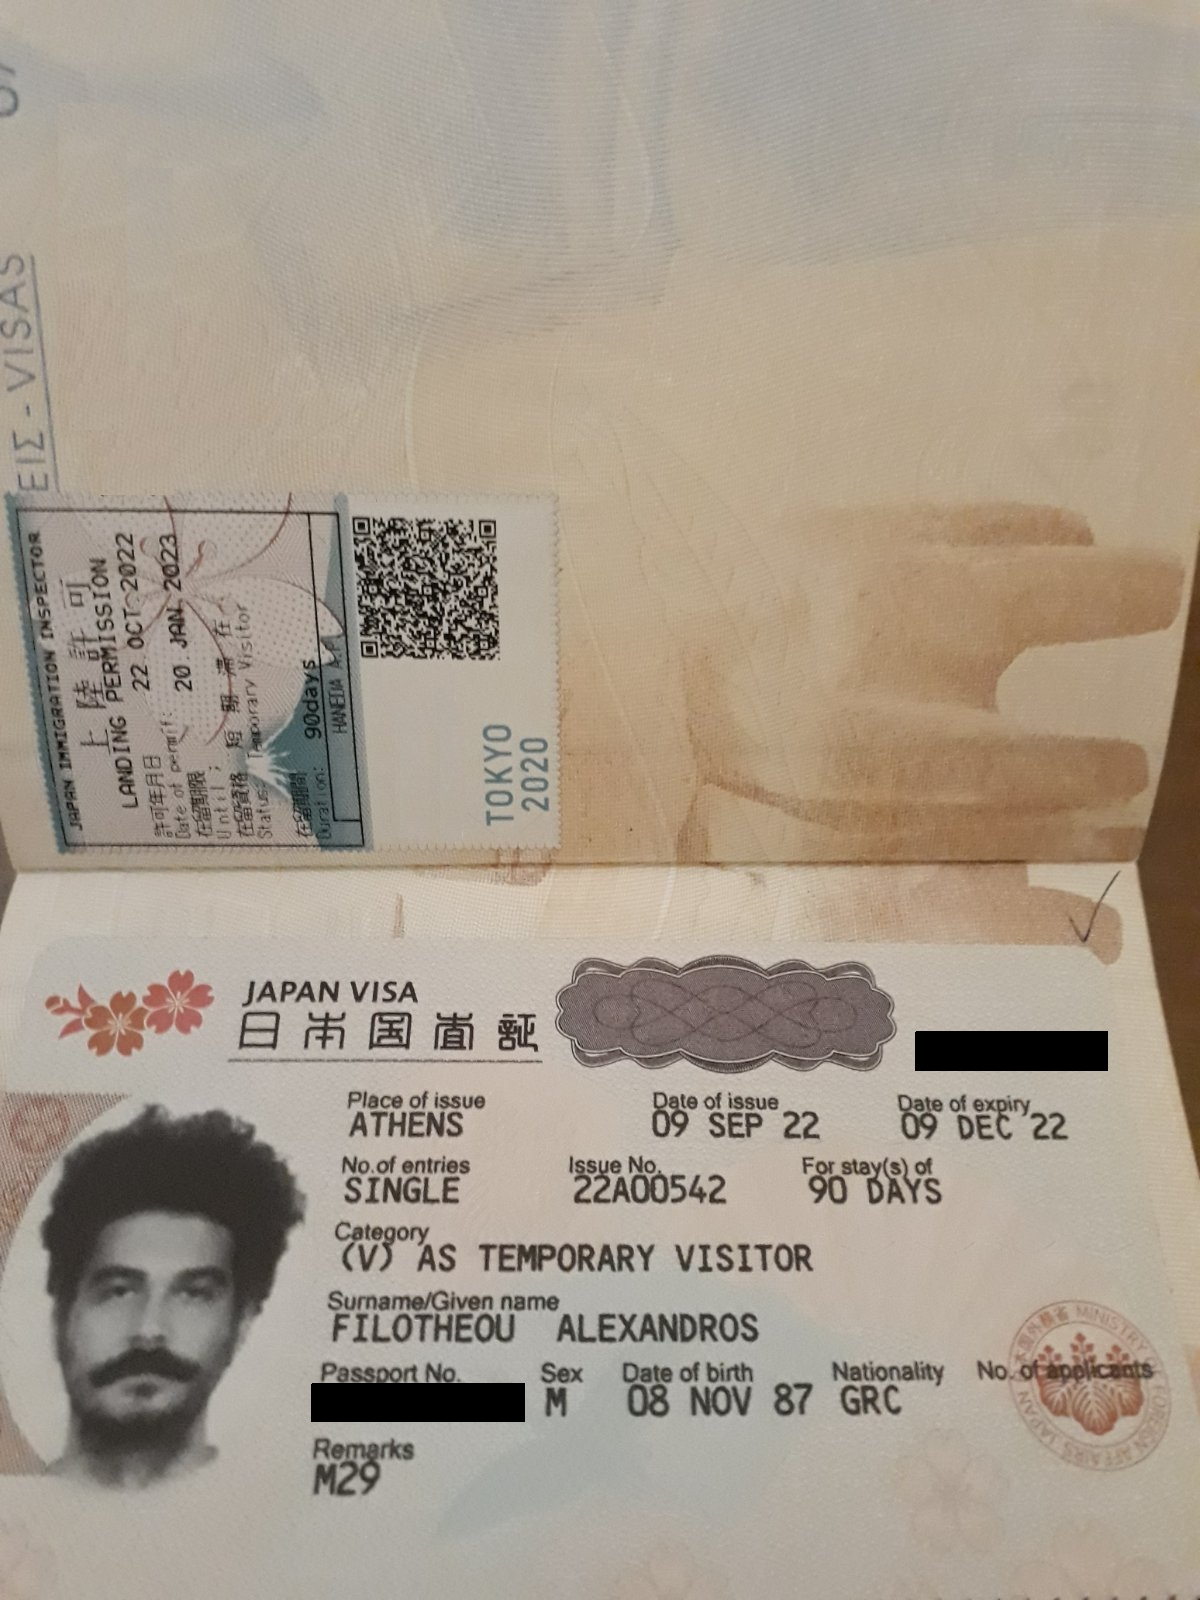
\includegraphics[scale=0.25]{./figures/parts/appendix/chapters/06/visa.jpg}
\end{figure}
%%%%%%%%%%%%%%%%%%%%%%%%%%%%%%%%%%%%%%%%%%%%%%%%%%%%%%%%%%%%%%%%%%%%%%%%%%%%%%%%
\begin{figure}[H]\centering
  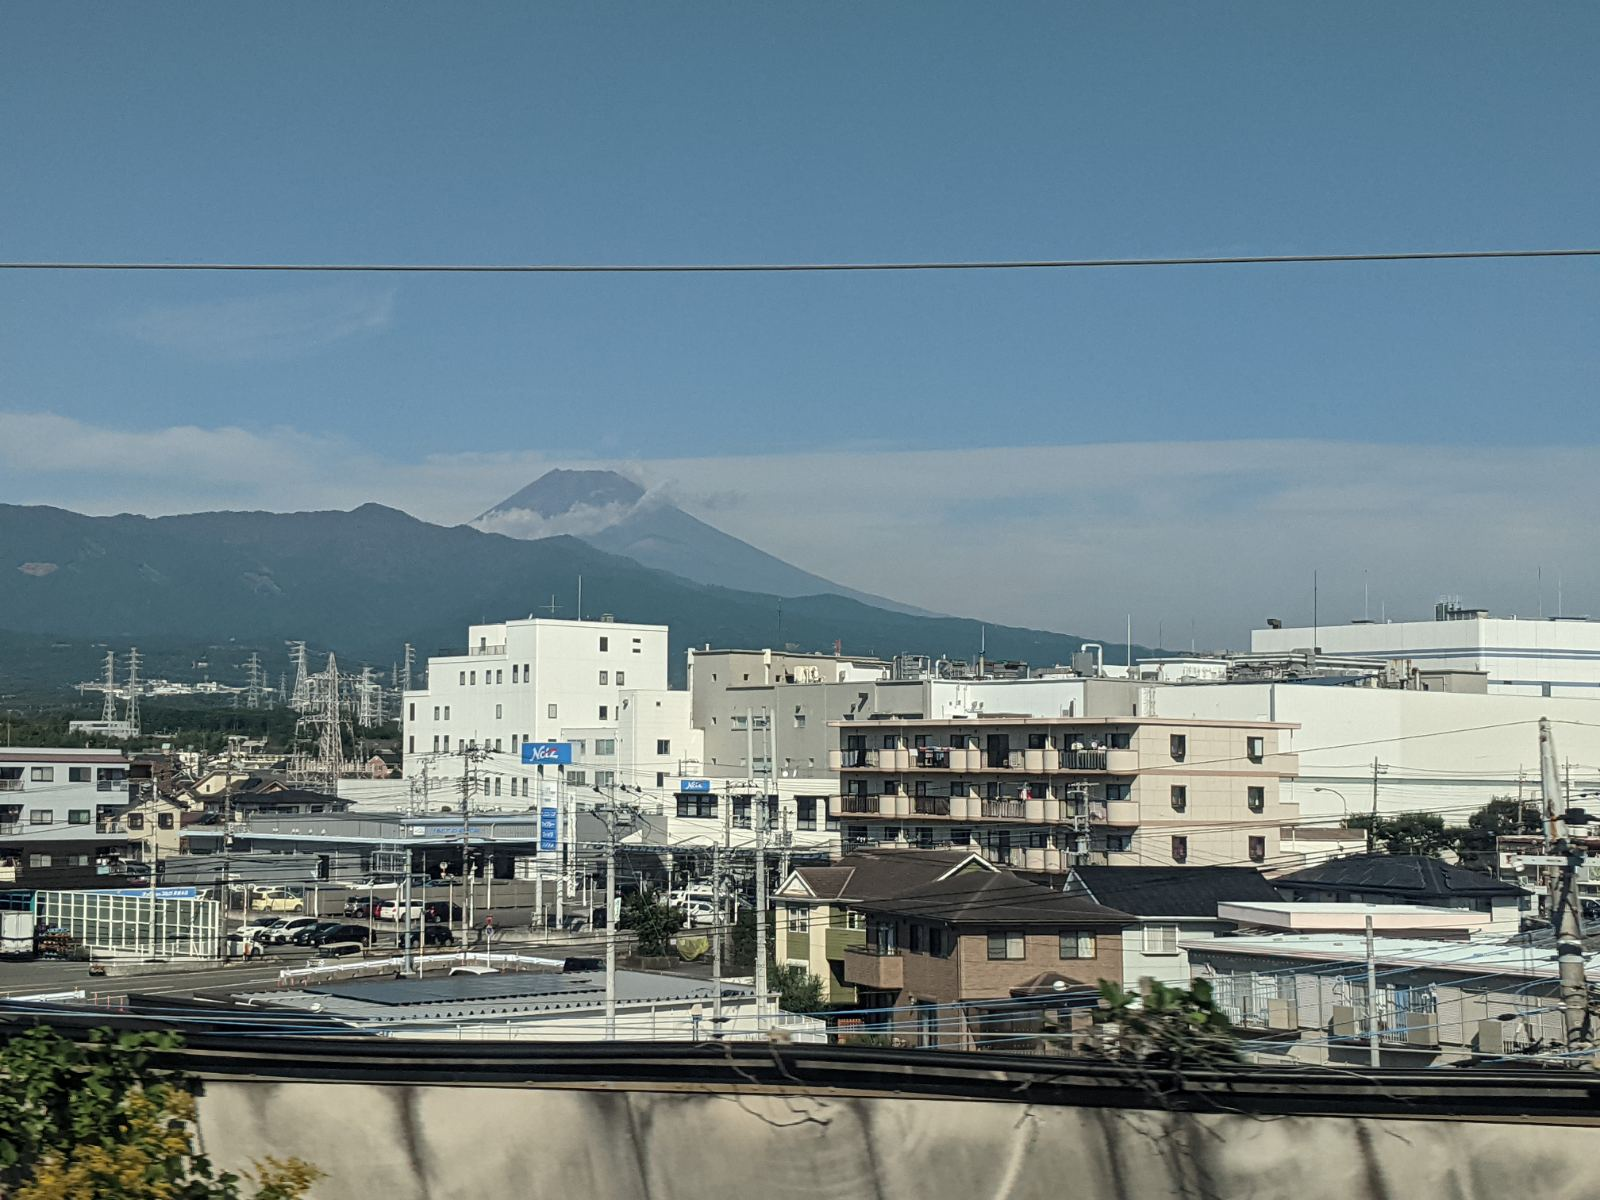
\includegraphics[scale=0.25]{./figures/parts/appendix/chapters/06/fuji_from_train.jpg}
\end{figure}
%%%%%%%%%%%%%%%%%%%%%%%%%%%%%%%%%%%%%%%%%%%%%%%%%%%%%%%%%%%%%%%%%%%%%%%%%%%%%%%%
\begin{figure}[H]\centering
  \includegraphics[scale=1]{./figures/parts/appendix/chapters/06/place_at_kyoto.jpg}
\end{figure}
%%%%%%%%%%%%%%%%%%%%%%%%%%%%%%%%%%%%%%%%%%%%%%%%%%%%%%%%%%%%%%%%%%%%%%%%%%%%%%%%
\begin{figure}[H]\centering
  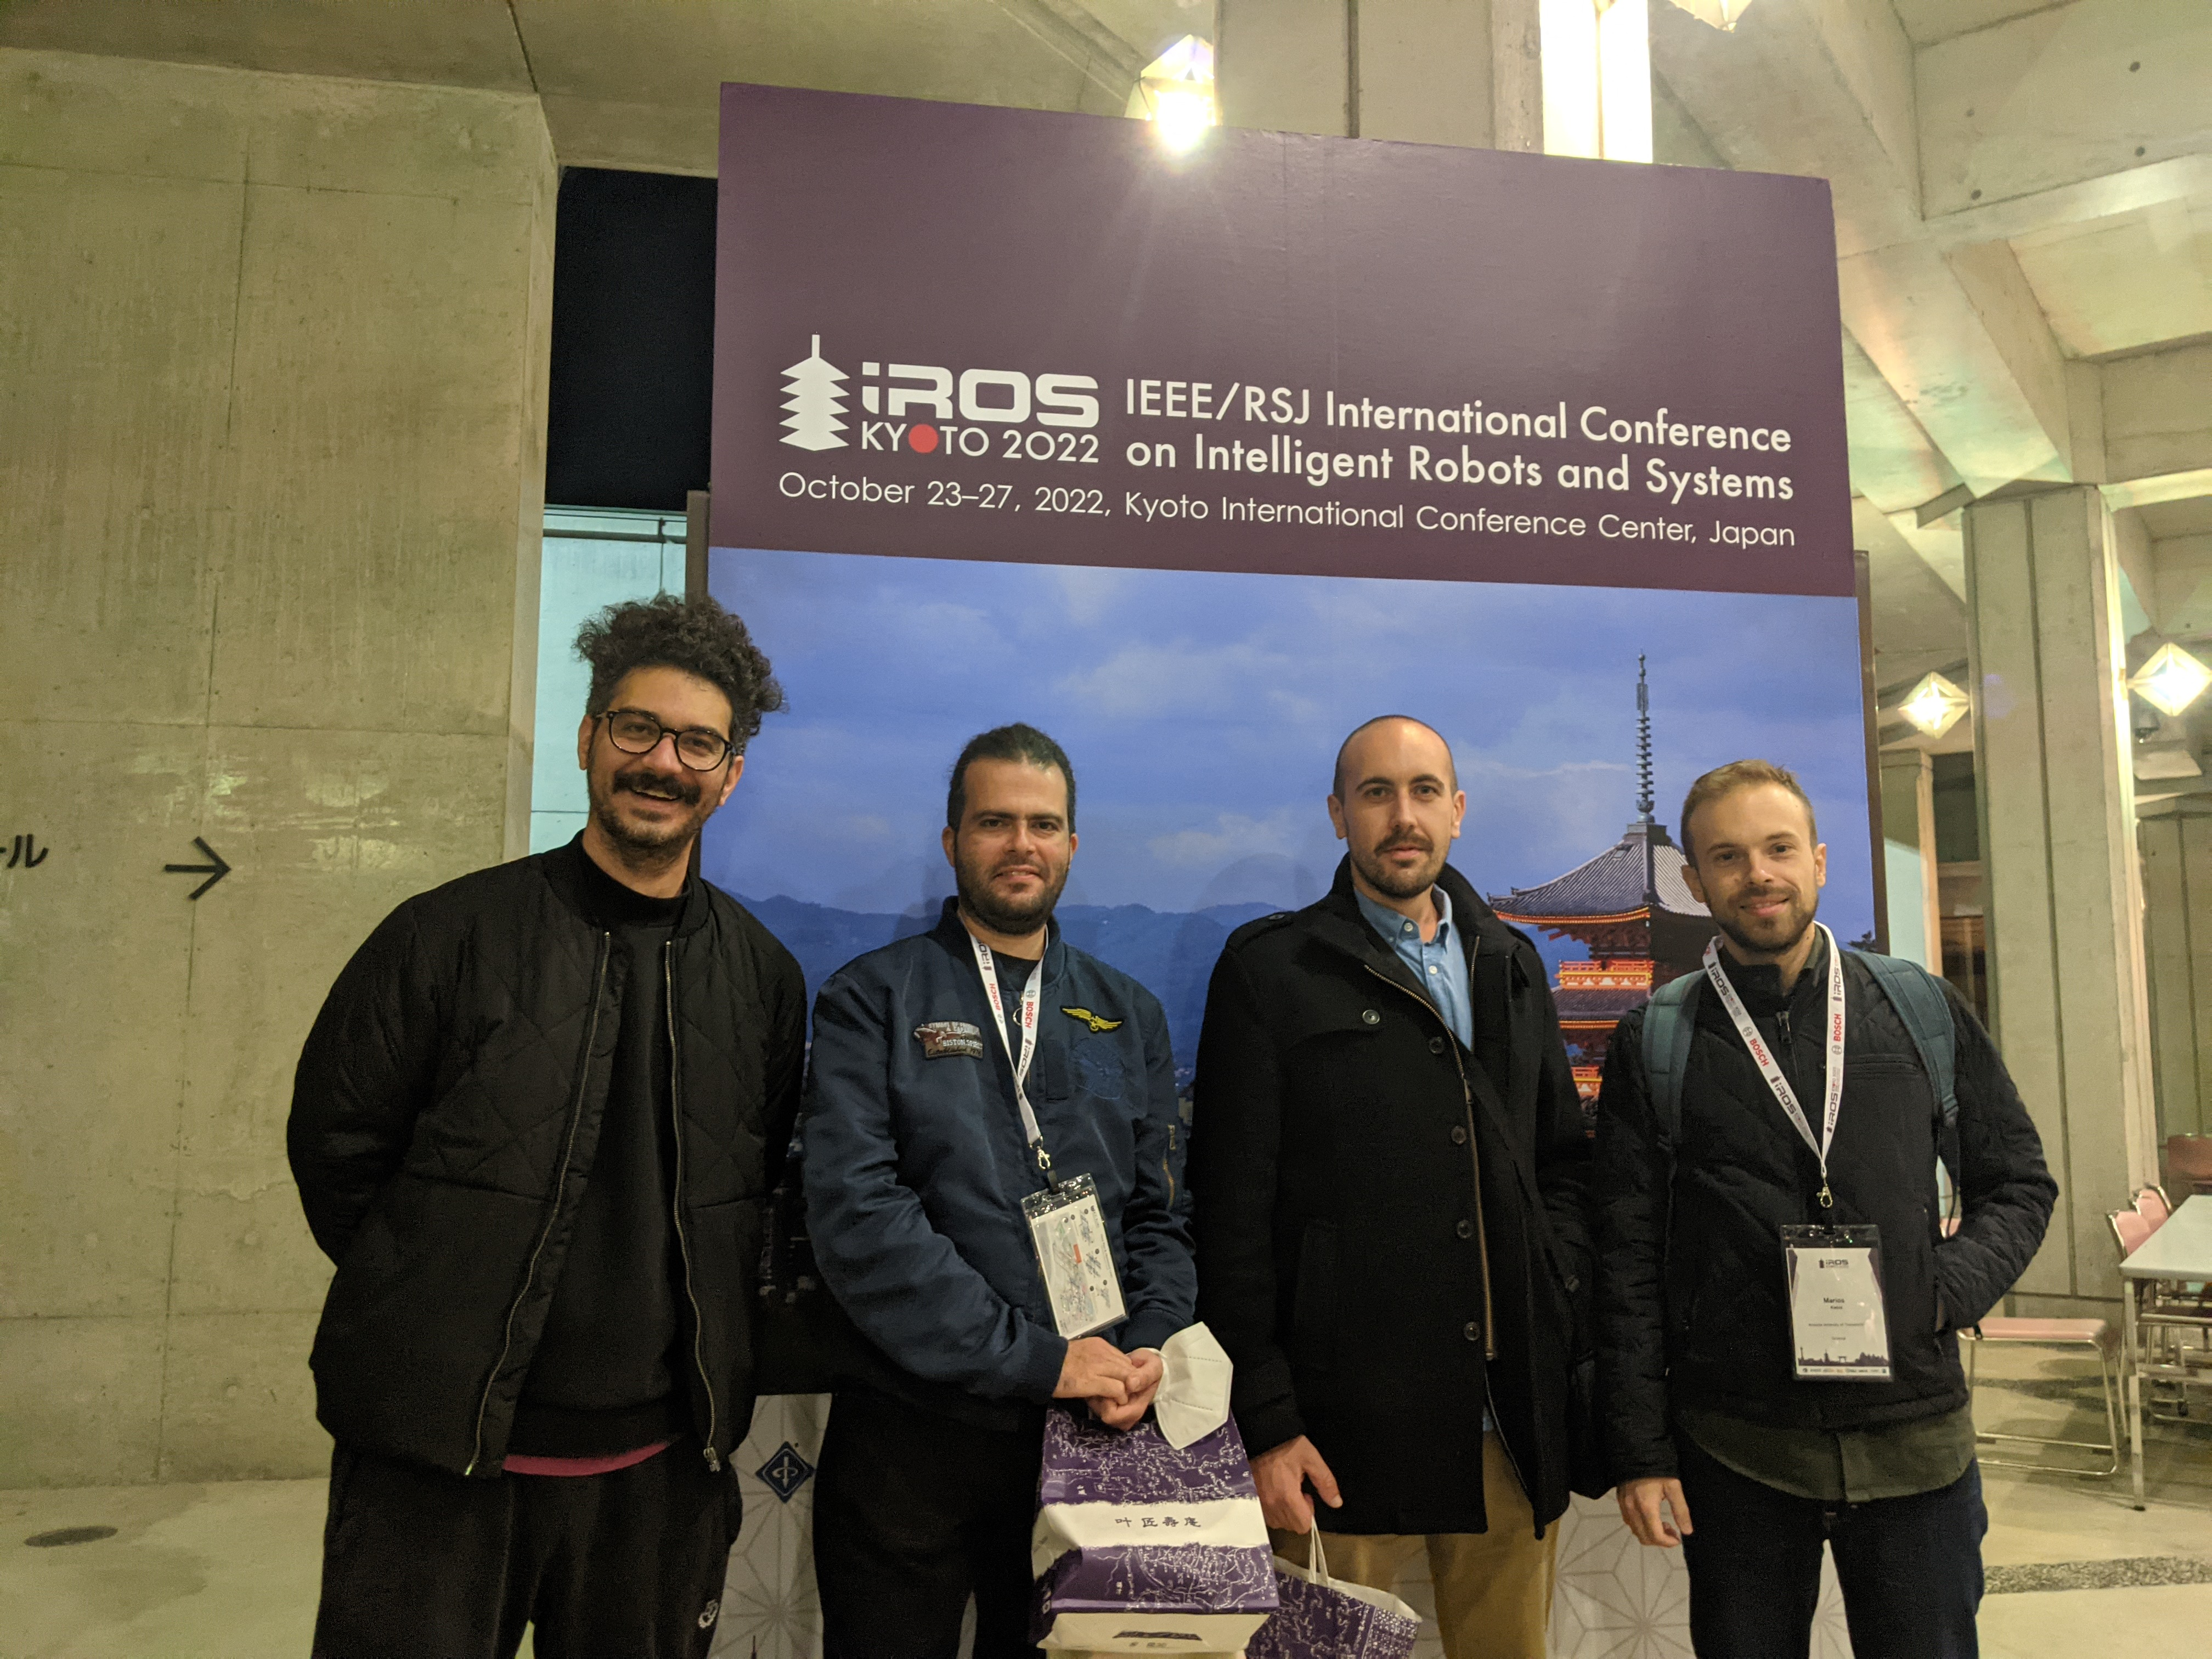
\includegraphics[scale=0.1]{./figures/parts/appendix/chapters/06/at_iros2022.jpg}
  \caption{\small Στο Διεθνές Συνεδριακό Κέντρο του Κυότο, όπου έκανα την πρώτη
           μου παρουσίαση \cite{Filotheou2022i}. Από αριστερά προς δεξιά:
           Αλέξανδρος Φιλοθέου, Λεωνίδας Δρούκας, Σωτήρης Σταυρίδης, Μάριος Κιάτος}
\end{figure}


%%%%%%%%%%%%%%%%%%%%%%%%%%%%%%%%%%%%%%%%%%%%%%%%%%%%%%%%%%%%%%%%%%%%%%%%%%%%%%%%
\section{Χωρίς θέμα}
%%%%%%%%%%%%%%%%%%%%%%%%%%%%%%%%%%%%%%%%%%%%%%%%%%%%%%%%%%%%%%%%%%%%%%%%%%%%%%%%
\begin{figure}[H]\centering
  \includegraphics[scale=1]{./figures/parts/appendix/chapters/06/phd_view.jpg}
  \caption{\small Η θέα από το γραφείο εκπόνησης}
\end{figure}
%%%%%%%%%%%%%%%%%%%%%%%%%%%%%%%%%%%%%%%%%%%%%%%%%%%%%%%%%%%%%%%%%%%%%%%%%%%%%%%%
\begin{figure}[H]\centering
  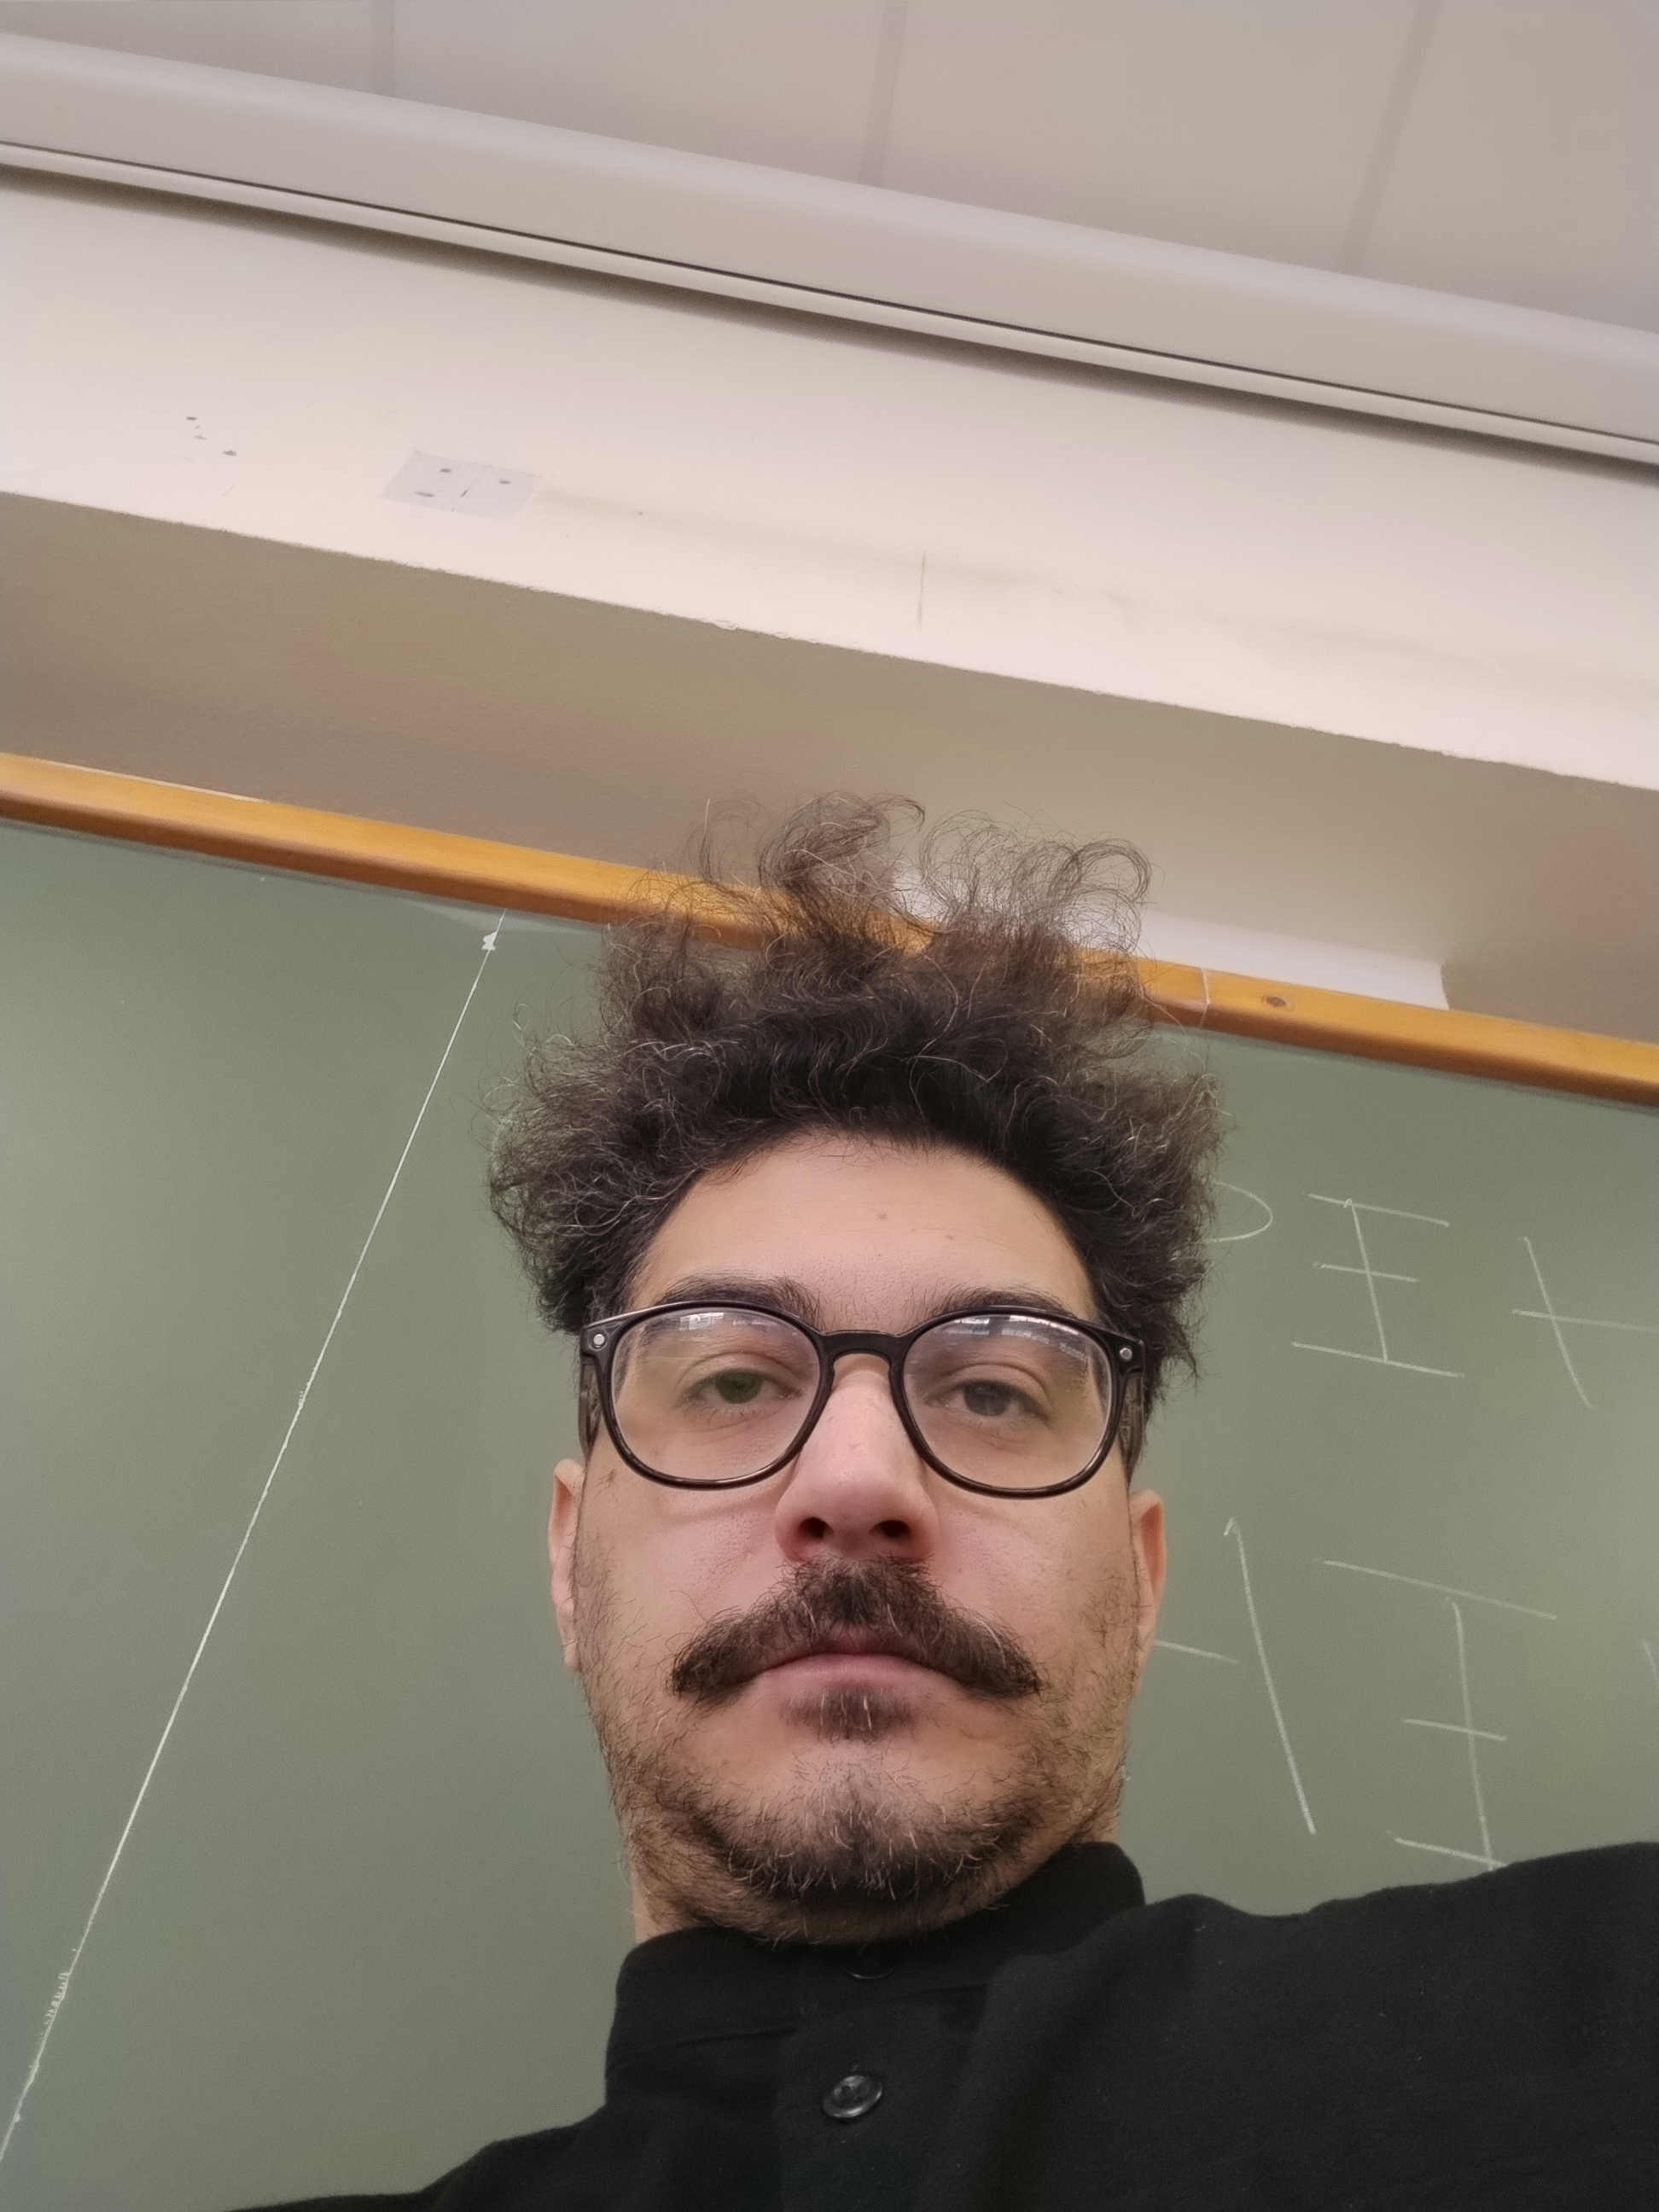
\includegraphics[scale=0.15]{./figures/parts/appendix/chapters/06/epitirisi.jpg}
  \caption{\small Κατά τη διάρκεια άσκησης του καθήκοντος της επιτήρησης
           μαθήματος το 2022}
\end{figure}
